\documentclass[a4paper,12pt,twoside]{report}
\usepackage[left=2cm,right=2cm,top=2cm,bottom=3cm]{geometry}

\usepackage{graphicx}				% Use pdf, png, jpg, or eps§ with pdflatex; use eps in DVI mode
\usepackage{amsmath}
\usepackage{multicol}
\usepackage{amssymb}
% \setlength\intextsep{11pt}
\usepackage{braket}
\numberwithin{equation}{section}
\usepackage{bm}
\usepackage{yfonts}
\usepackage{lipsum}
\usepackage{microtype}
\usepackage{appendix}
\usepackage{soul}
\usepackage{titlesec}
\usepackage{hyperref}
\usepackage{bbm}
\usepackage{titlesec}
\usepackage{subfiles}
\usepackage{tikz}
\usepackage{wrapfig}
\usepackage[justification=centering]{caption}

% \usepackage[sectionbib]{chapterbib}

\usepackage{verbatim}
\usepackage{latexsym}
\usepackage{setspace}

\input{uhead.sty}
\pagestyle{empty}

% \setlength{\parskip}{2ex plus 0.5ex minus 0.2ex}
% \setlength{\parindent}{0pt}
% \linespread{1.5}

\makeatletter  %to avoid error messages generated by "\@". Makes Latex treat "@" like a letter

\def\submitdate#1{\gdef\@submitdate{#1}}

\def\maketitle{

  \begin{titlepage}{
    % \linespread{1.5}
    
    \Large University of London \\
    %\linebreak
    Imperial College of Science, Technology and Medicine \\
    %\linebreak
    Department of Physics
    \rm
    \vskip 3in
    \Large \bf \@title \par
  }
  \vskip 0.3in
  \par
  {\Large \@author}
  \vskip 4in
  \par
  Submitted in part fulfilment of the requirements for the degree of 
  \linebreak
  Doctor of Philosophy in Physics of Imperial College of Science,  
  \linebreak
  Technology and Medicine, \@submitdate
  \vfil
  \end{titlepage}
}

\def\titlepage{
  \newpage
  \centering
  \linespread{1}
  \normalsize
  \vbox to \vsize\bgroup\vbox to 9in\bgroup
}
\def\endtitlepage{
  \par
  \kern 0pt
  \egroup
  \vss
  \egroup
  \clearpage
}

\def\abstract{
  \begin{center}{
    \large\bf Abstract}
  \end{center}
  \small
  %\def\baselinestretch{1.5}
  \linespread{1.0}
  \normalsize
}
\def\endabstract{
  \par
}

\newenvironment{acknowledgements}{
  \clearpage
  \begin{center}{
    \large \bf Acknowledgements}
  \end{center}
  \small
  \linespread{1.5}
  \normalsize
}{\clearpage}
\def\endacknowledgements{
  \par
}

\newenvironment{dedication}{
  \clearpage
  \begin{center}{
    \large \bf Dedication}
  \end{center}
  \small
  \linespread{1.5}
  \normalsize
}{\clearpage}
\def\enddedication{
  \par
}

\def\preface{
    \pagenumbering{roman}
    \pagestyle{plain}
    % \doublespacing
}

\def\body{
    \clearpage    
    \pagestyle{uheadings}
    \tableofcontents
    \pagestyle{plain}
    % \clearpage
    % \pagestyle{uheadings}
    % \listoftables
    % \pagestyle{plain}
    \clearpage
    \pagestyle{uheadings}
    \listoffigures
    \pagestyle{plain}
    \clearpage
    \pagestyle{uheadings}
    \pagenumbering{arabic}
    % \doublespacing
}

\makeatother  %to avoid error messages generated by "\@". Makes Latex treat "@" like a letter
\input{boxit.sty}
\input{blocked.sty}




\hypersetup{
    colorlinks,
    citecolor=black,
    filecolor=black,
    linkcolor=black,
    urlcolor=black
}

\newcommand{\normallinespacing}{\renewcommand{\baselinestretch}{1.5} \normalsize}
\newcommand{\mediumlinespacing}{\renewcommand{\baselinestretch}{1.2} \normalsize}
\newcommand{\narrowlinespacing}{\renewcommand{\baselinestretch}{1.0} \normalsize}

%Define that shaded box you like
\usepackage[noframe]{showframe}
\usepackage{framed}
\renewenvironment{shaded}{%
    % \everypar={{\setbox0=\lastbox}\everypar{}}
  \def\FrameCommand{\fboxsep=\FrameSep \colorbox{shadecolor}}%
  \MakeFramed{\advance\hsize-\width \FrameRestore\FrameRestore}}%
 {\endMakeFramed}
\definecolor{shadecolor}{gray}{0.9}


% math commands:
\newcommand*{\vertbar}{\rule[-1ex]{0.5pt}{2.5ex}}
\newcommand*{\horzbar}{\rule[.5ex]{2.5ex}{0.5pt}}
\newcommand{\dline}[1]{\underline{\underline{#1}}}

\newcommand{\tr}{\ensuremath{\textup{Tr}}}
\newcommand{\1}{\ensuremath{\mathbbm{1}}}
% \renewcommand{\bf}[1]{\ensuremath{\textbf{#1}}}
\newcommand{\re}{\ensuremath{\textup{Re}}}
\newcommand{\im}{\ensuremath{\textup{Im}}}
\newcommand{\ts}{\textsuperscript}
\renewcommand{\r}{\ensuremath{\textbf{r}}}
\newcommand{\jon} {J_{\textup{on}}}
\newcommand{\joff} {J_{\textup{off}}}



\begin{document}

\title{\LARGE {\bf I Simply Cannot, and Will Not, Stop Shagging the Kitaev Model}\\
 \vspace*{6mm}
}

\author{Peru d'Ornellas} 
\submitdate{December 2023}
\narrowlinespacing

\maketitle



\begin{abstract}

    bunch of bloody shite this isnt it...
    
\end{abstract}

\tableofcontents

\pagestyle{uheadings}
\chapter{Introduction}


\pagenumbering{arabic}

In 1928, just two years after Erwin Schr\"odinger published his famous wave equation, Felix Bloch\footnote{At the age of 24} proposed a new method for calculating the electronic properties of solids. By this point, the idea that electrons in atoms arranged themselves into a hierarchy of discrete orbitals was well-established. Bloch proposed that, rather than starting with a free electron and considering how its motion might be affected by the potential in a material, the properties might be better understood by starting with a set of electronic states $\ket{\phi_n(\textbf{R}_i)}$, corresponding to the $n^{\textup{th}}$ orbitals on the atom at position $\textbf{R}_i$. Here, a wavefunction could be constructed by taking a linear combination of these orbitals. Next, the Hamiltonian operator, given by 
\begin{align} \label{eqn:schrodinger_H}
    H = \frac{\textbf{p}^2}{2m} + V
\end{align}
would be rewritten in terms of these states. By exploiting the translational symmetry in crystalline materials and considering only the lowest energy $s$ orbital, Bloch was able to solve the periodic Schr\"odinger equation and the technique -- known as the LCOM (linear combination of atomic orbitals), or tight-binding method -- paved the way for the development of band theory.

In practice, this was a spectacularly complex procedure to perform rigorously. To re-express the Hamiltonian in terms of orbitals, one had to evaluate an enormous number of integrals of the form $\braket{\phi_n(\textbf{R}_i)|H|\phi_m(\textbf{R}_j)}$ -- one for each pair of orbitals separated by each lattice translation. Thus, finding the exact form of the Hamiltonian was considered an impossible task. Rather, the utility of this method became apparent when one accepted this impossibility and just guessed the form of $H$. With just a few assumptions one could simplify the Hamiltonian to the point that it depended on only a small number of parameters. For example, one would expect the coupling between two orbitals to vanish unless they were sufficiently close as to overlap. Furthermore, by studying the symmetries in a crystalline material, one finds many couplings that must be equivalent. Thus, the game of constructing a tight binding model for a particular material became one of adjusting this small number of parameters until the model matched the properties found in experiment.

Although we started with the original form of Schr\"odinger's Hamiltonian (eqn.~\ref{eqn:schrodinger_H}), the tight-binding picture we have arrived at is a radically different world for an electron to live in. In Schr\"odinger's story, the electron exists as a wave in a fundamentally smooth world, where the potential defines a landscape through which the electron roams. However, in Bloch's story the collective properties of the electrons emerge from the overlap between a discrete lattice of orbitals. Here the landscape is more akin to an archipelago of islands, with electrons that can hop from island to island as in fig.~\ref{fig:hopping_electron}. Constructing a model in this formalism is a completely different procedure, since one must first determine the shape of the lattice -- the geography of the islands -- and only then can we build a Hamiltonian and write down the equations of motion.

\begin{figure}
    \centering
    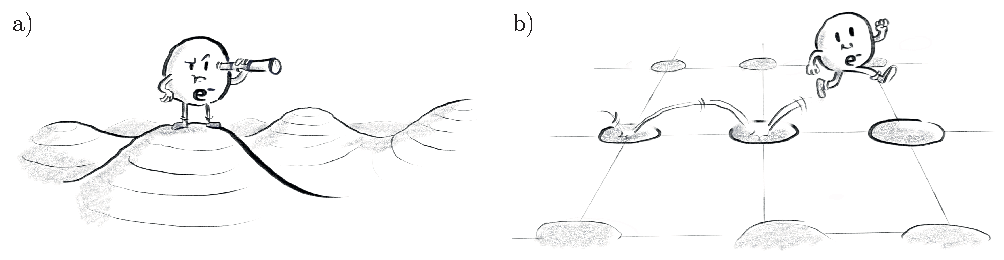
\includegraphics{introduction/figures/hopping_electron.pdf}
    \caption{
    \textbf{(a)} 
    \textbf{(b)} . 
    } 
    \label{fig:hopping_electron}
\end{figure}


% % Since the dawn of time man has gazed upon the universe and searched for answers. Some of these answers proved simple, revealing themselves after just a brief investigation. Some answers only appeared after hundreds, even thousands of years of study, passed on from generation to generation, and some answers have evaded discovery for all of time. This thesis is concerned with one of the latter questions, namely: \textit{How do the topological properties of electronic phases of matter depend on lattices upon which they are constructed?}

% % Rough opening remarks:

% When learning quantum mechanics, one's first introduction to the nature of the electron often comes in the form of the Schr\"odinger equation for a free particle:
% \begin{align}
%     i\frac{\partial}{\partial t} \ket \psi = \frac{\textbf p ^2}{2m} \ket{\psi}.
% \end{align}
% Here the electron exists as an isolated object, wandering a smooth empty expanse. Perhaps, with the addition of a potential $V$, this environment may become populated with objects, forces or even other electrons with whom to interact. Starting with this picture, one is invited to view the world inhabited by these particles as a (sometimes strong) perturbation away from a smooth and uniform place. In many branches of physics this remains a helpful story, after all -- as far as we know -- the world \textit{is} smooth and mostly empty.  

% However, for an electron that lives in a solid this picture can be deeply misleading. Here the shape of the landscape -- defined by the arrangement of atoms and the presence of other electrons -- can be the most important factor in defining the properties of the system. In many materials, the potential well at each atom is sufficiently deep that electrons remain tightly confined to them. Thus our smooth and continuous world is broken up into a set of islands, each hosting a collection of localised states that can be inhabited. Now, collective electronic properties emerge from the overlap between these localised states -- allowing the electrons to hop from site to site, or realign their spin and internal degrees of freedom in response to the state of a neighbour. In the most extreme example, the electron-electron repulsion can be strong enough that electrons are completely forbidden from hopping from one atom to a neighbour -- forming a so-called Mott insulator \cite{mott_basis_1949}. 


% Thus, rather than treating the environment as a potential in a smooth world, it is more useful to view the electrons as moving between a set of isolated islands arranged on the vertices of a discretised lattice defined by the background material. This intuition forms the 

% % tight-binding model, where the equations of motion are built on the assumption that electrons exist only on a discretised lattice defined by the background material. 
% % Finally, in certain materials, the electron-electron interaction is such that electrons are immobilised at each site -- mott insulators -- and the system has truly separated into a lattice of individual sites hosting individual electrons, interacting with one another primarily through the overlap of their wavefunctions. 
% % In the weak limit this background can be seen as a gentle perturbation on the motion of an otherwise free particle, however in many materials the opposite is true -- the electronic properties of the material are formed by the overlap of outer orbitals in the atoms, and the lattice can be seen rather as fundamental in defining the ways electrons can exist inside a material. Here the electrons are strongly localised to individual atoms, or can jump from atom to atom, and is described by a tight binding model -- viewing each atom as a site that can hold number of electrons in well-defined states. 

% In these materials, where electrons are constrained in their movement by the structure of their hosting material, an understanding of their collective properties requires two ingredients: The microscopic interactions that describe how electrons interact with their surroundings and each other, and the geometry of the lattice on which they live. Thus, a natural question to ask is `How does the shape of these lattices affect the ways that electrons can order within them'. It is this question that motivates 

% Historically, this question this has proved to be an extremely rich question, with an astonishing variety of answers depending on the material and the microscopic interaction terms. 

% There are examples of materials where the properties of the electron phases are remarkably insensitive to lattice geometry, and the same type of Hamiltonian defined on any lattice will produce largely the same physics. A rather obvious example are ferromagnetic materials, where the spins forming the material will align regardless of the microscopics of the lattice. Even on different lattices, the Ising model has been shown to have identical behaviour in the thermodynamic limit, where the universality class remains unaffected by local changes in lattice. More recently, a new class of remarkably insensitive phenomena emerged -- the quantum Hall effect. Here, the bulk conductance of the electrons is quantised to a precise value, regardless of the presence of disorder in the system. Here, the Hamiltonian defined on any lattice will have largely the same properties and the presence of disorder serves not to disrupt but to stabilise the universal nature of these materials properties. 

% At the other extreme are materials where the same Hamiltonian defined on different lattices can give wildly different results. An example is the antiferromagnetic Heisenberg model, which can give N\'eel, VBS and was even proposed as a possible spin liquid phase on a sufficiently geometrically frustrated lattice. 

\section{Universality} \label{sec:universality}

The search for universal properties, i.e. those that are insensitive to the microscopic details of matter, is an old one. At the atomic level the world is spectacularly complex, with an enormous number of constituent particles interacting with one another in ways that are chaotic and poorly understood. Yet, by the time we reach the macroscopic scale, most of these complexities have been averaged away, and a familiar world emerges. One of the remarkable aspects of this averaging is that different microscopic systems converge to the same macroscopic behaviour. For example, despite enormous variation in chemical composition, all liquids have similar bulk properties, and follow almost identical equations of motion, \textit{more is the same}.% \cite{anderson_more_1972}. 

One of the great successes in understanding this universality was developed in the mid 20th century, starting with the work of Ginzburg and Landau \cite{ginzburg_theory_1950}, and then further developed by a generation of physicists, most notably Ken Wilson \cite{wilson_renormalization_1975} who introduced the concept of the renormalisation group (RG). Let us briefly sketch the central idea using the Ising model as an example, although a thorough discussion is beyond the scope of this thesis, and can be found in Refs.~\cite{cardy_scaling_1996,chaikin_principles_1995}. 

We start with a set of classical spin $\{s_i\}$ arranged on a lattice, interacting according to a general Hamiltonian, for example the Ising Hamiltonian,
\begin{align}
    H = -B \sum_{j} s_j - J \sum_{\braket{jk}} s_j s_k.
\end{align}
Rather than working with individual spins, which can only take two values $\pm 1$, Ginzburg and Landau suggested constructing a smoothly varying local order parameter $m(\textbf x)$ by dividing up these spins into blocks and averaging over each block as seen in Fig.~\ref{fig:rg_flow}a. In this language, the partition function for the model can be rewritten in terms of a path integral over this order parameter
\begin{align}
    \mathcal Z = \sum_{\{s_i\}} e^{-\beta E(s_i)} 
    \rightarrow 
    \int \mathcal D m \sum_{\{s_i\}|m(\textbf x)} e^{-\beta E(s_i)}.
\end{align}
The sum on the right-hand side is arbitrarily difficult, however -- as with tight binding a few decades earlier -- the key insight was that we didn't have to evaluate it at all, rather we could just wrap the quantity up as some unknown free energy
\begin{align}
    \sum_{\{s_i\}|m(\textbf x)} e^{-\beta E(s_i)} = e^{- \beta F(m)},
\end{align}
and make a guess as to the form of the free energy by considering only coefficients that are consistent with the symmetries of the system, for example in an Ising model with no external field, the system has spin-flip symmetry -- so odd powers of $m$ are forbidden,
\begin{align}
    F(m) = \int d^dx 
    \left [ 
    \gamma (\nabla m)^2 
    + \alpha_2 m^2 +  \alpha_4 m^4 + ...
    \right ].
\end{align}
Thus, we have parametrised every possible effective theory for our model with a (possibly infinite) set of prefactors, $\{\gamma, \alpha_n\}$. The next insight came by considering how an effective theory might change under a \textit{rescaling transformation}. There are many ways that this transformation may be formulated, for example one might consider a real-space method, where $m(\textbf x)$ is redefined by choosing some larger block size and averaging $m(\textbf x)$ over this area, effectively zooming out and setting a limit to how finely-resolved the fluctuations in the model can be, shown in Fig.~\ref{fig:rg_flow}b. Equivalently, one can consider imposing a momentum cut-off in the partition function, and integrating out the high momentum modes that correspond to the unwanted small-scale fluctuations. Parametrising this scaling with $\tau$, we find that the coefficients of the free energy pick up a $\tau$-dependence and the rescaling process generates a flow in parameter space $\{\gamma, \alpha_n\} \rightarrow \{\gamma(\tau), \alpha_n(\tau)\}$.
\begin{figure}
    \centering
    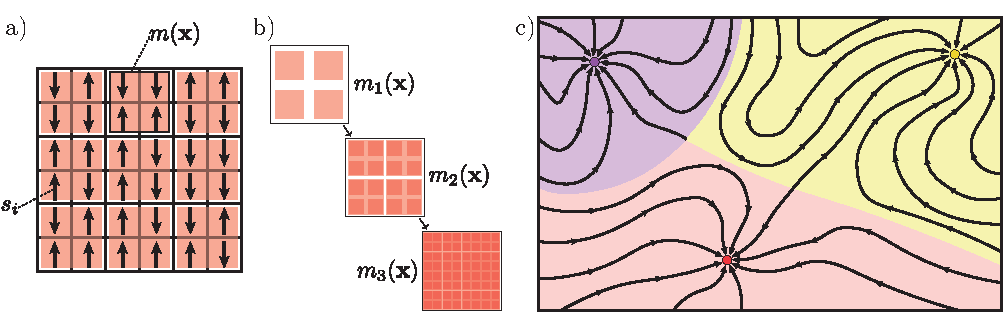
\includegraphics{introduction/figures/rg_flow.pdf}
    \caption[Illustration of a spin-averaging procedure and real space renormalisation step. Diagram of theory space, with a set of stable fixed points.]{
    \textbf{(a)}~In the first step of coarse graining, an averaged magnetisation parameter $m(\textbf x)$ is constructed by choosing and averaging over set of spins $s_i$, each set is indicated with a red box.
    \textbf{(b)}~A real space rescaling can be performed by averaging over successively larger chunks of spins, leading to a set of successively more coarse-grained order parameters $m_i(\textbf x)$. 
    \textbf{(c)}~A heuristic diagram of a parameter space for $F(m)$, where arrows indicate the flow under RG. In each region, the theory flows to one corresponding fixed point, indicated with a circle, which defines the long-range properties of the model. 
    } 
    \label{fig:rg_flow}
\end{figure}

Under this transformation, the points where the free energy functional is static correspond to fixed points where the effective theory becomes scale-invariant, since any dependence on scale implies that the model will change under $\tau$. Remarkably, for many models of interest there turns out to be only a finite number of these fixed points. Under RG flow many microscopically different systems, which start from different points in parameter space, flow to the same fixed point and thus have the same long-range properties, a diagram is shown in Fig.~\ref{fig:rg_flow}c. Thus, the whole of parameter space can be divided into a set of regions, where starting at any point in that region will always flow to the same fixed point, and thus have the same long-range effective description. Thus, any microscopic change to the model, provided that the change does not alter the symmetries of the model, will only have the effect of perturbing the starting point in RG. If this perturbation doesn't move us out of one region and into another, we have the guarantee that the long-range properties of the system are unaffected.

\subsection{The Integer Quantum Hall Effect and Chern Number} \label{sec:qhe}

\begin{figure}
    \centering
    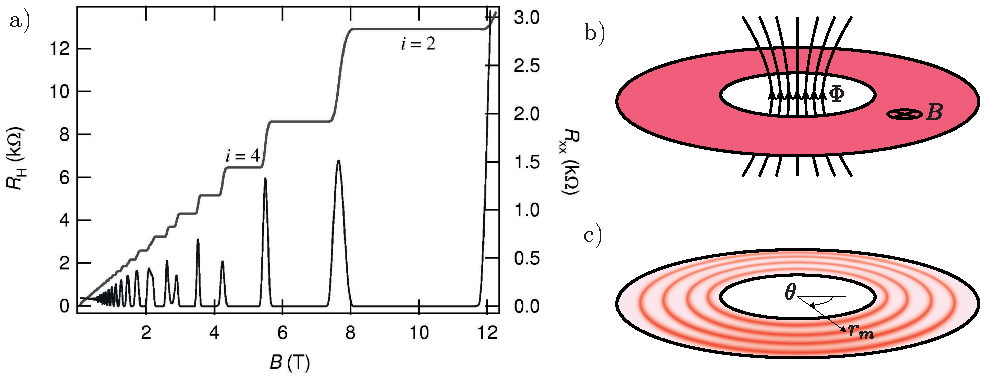
\includegraphics{introduction/figures/QHE.pdf}
    \caption[Hall conductivity as a function of applied magnetic field. A Corbino disc geometry with a sketch of successive states within a Landau level.]{ 
        \textbf{(a)}~The measured resistivity in a GaAs heterostructure at $0.1$ K. \textit{Figure reproduced from \cite{jeckelmann_quantum_2003}.}
        \textbf{(b)}~The geometry proposed by Halperin \cite{haplerin_quantized_1982}. Here a 2D electron gas is confined to the ring, pierced by a transverse magnetic field parametrised by $B$. A flux given by $\Phi$ is threaded through the centre of the ring, which adiabatically increased from $\Phi = 0 \rightarrow \Phi_0$.
        \textbf{(c)}~Depiction of a set of wavefunctions that form part of the lowest Landau level. The $m^{\textup{th}}$ wavefunction is localised to a ring with radius $r_m$. 
    } 
    \label{fig:hall_conductivity}
\end{figure}

In the early 1980s a very different form of universal physics was emerging at the National Laboratory for Intense Magnetic Fields in Grenoble. Here, Klaus von Klitzing was studying the transverse Hall conductivity in silicon-based MOSFETs (metal-oxide-semiconductor field-effect transistor) prepared by Gerhard Dorda and Michael Pepper. These transistors allowed von Klitzing to prepare electrons in a nearly ideal 2D gas at extremely low temperatures and under high magnetic fields. Here, rather than finding the linear relationship between transverse resistivity and applied field predicted by classical Drude theory, von Klitzing found that the transverse resistivity contained a set of plateaux at precisely quantised values given by
\begin{align} \label{eqn:hall_conductivity}
    \rho_{xy} = \frac{2\pi \hbar}{e^2 \nu}, \ \nu\in \mathbb Z,
\end{align}
as shown in Fig.~\ref{fig:hall_conductivity}a \cite{klitzing_new_1980,klitzing_quantizes_1986}. This quantisation was extremely precise, accurate to one part in $10^6$ and has since been adopted as the standard for defining the unit of resistance ($\Omega$) \cite{jeckelmann_quantum_2003}. The precision is particularly surprising given that the samples von Klitzing was using contained fairly substantial disorder. In fact, as we shall see in the following discussion, the presence of some disorder is necessary for producing the sharp jumps in conductivity seen here. 

One of the first steps towards understanding the precise quantisation of the Hall conductivity was proposd by Laughlin \cite{laughlin_quantized_1981}, and developed by Halperin \cite{haplerin_quantized_1982} who considered a quantum Hall system constructed on a ring geometry as shown in Fig.~\ref{fig:hall_conductivity}b. The Hall conductivity could be tested by adiabatically threading some quantity of flux $\Phi$ through the centre of the ring. Including the perpendicular magnetic field and working in symmetric gauge, the electrons experience a magnetic vector potential of the following form,
\begin{align}
    \textbf A = \left ( 
        \frac{1}{2} B r - \frac{\Phi}{2\pi r}    
     \right ) \hat{\bm \theta}.
\end{align}
After solving the Schr\"odinger equation for this potential, one finds the electrons organised into Landau levels (LLs) with energy determined by the cyclotron frequency, $E = \hbar \omega_c(\nu + 1/2)$. The lowest LL consists of a degenerate set of ring-like wavefunctions,
\begin{align}
    \psi_{LLL,m} \sim e^{im\theta} f(r - r_m),
\end{align}
shown in Fig.~\ref{fig:hall_conductivity}c. Here $f(r - r_m)$ is a Gaussian profile, such that the $m^{\textup{th}}$ state is localised to a ring whose radius is determined by the flux enclosed, according to 
\begin{align}
    B\pi r_m^2 = m \Phi_0 + \Phi,
\end{align}
where $\Phi_0 = 2 \pi \hbar / e$ is a single flux quantum. Thus, by adiabatically threading a single flux quantum through the ring (by slowly tuning $\Phi$ from $0 \rightarrow \Phi_0$), we have the effect of transforming each $r_m \rightarrow r_{m+1}$. Each state in the Landau level moves outwards, taking the place of its neighbour, a process known as \textit{spectral flow}. Once the process is complete, the system must be identical to before -- since a whole flux quantum can always be removed with a gauge transformation -- however now there is an extra electron on the outer edge and a missing electron on the inner edge. Thus, the ring behaves like a conveyor belt under flux insertion, transferring a single electron from the inside to the outside, as shown in Fig.~\ref{fig:hall_conductivity_disorder}c. To calculate the resistivity associated with this process, let us suppose the adiabatic process happened over some timescale $T$, and calculate the EMF,
\begin{align}
    \mathcal E = -\frac{\partial \Phi}{\partial t} = -\frac{\Phi_0}{T},
\end{align} 
and the current induced by the transfer of one electron,
\begin{align}
    I = -\frac e T,
\end{align}
giving an overall transverse resistivity of
\begin{align}
    \rho_{xy} = \frac{\mathcal E}{I} = \frac{\Phi_0}{e} = \frac{2\pi \hbar}{e^2}.
\end{align} 
This calculation was performed for a single Landau level; however, the story is straightforwardly transferable to the case when several Landau levels sit below the Fermi energy, since each level independently transports an electron from the inside to the outside edge. Thus, for $\nu$ Landau levels below the Fermi energy, we find an overall conductivity given by Eqn.~\ref{eqn:hall_conductivity}.

\begin{figure}
    \centering
    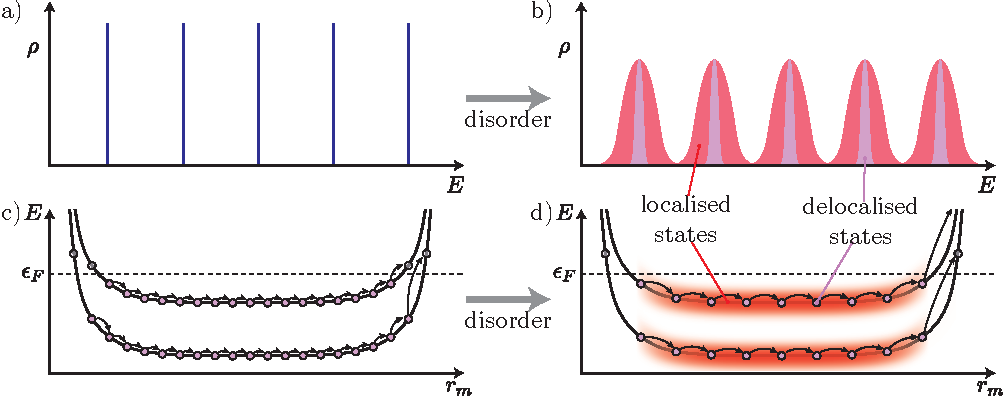
\includegraphics{introduction/figures/QHE_2.pdf}
    \caption[Density of states and energy of landau levels for both a clean and disordered quantum Hall sample on a ring geometry.]{
        \textbf{(a)}~Density of states for a set of five Landau levels in a clean system. Here all states in each LL are degenerate and delocalised around the ring. 
        \textbf{(b)}~In a disordered system, the Landau levels are broadened, and many states become localised. However, each LL still contains a central set of delocalised states.
        \textbf{(c)}~Energy of a set of two Landau levels as a function of radius, showing the effect of a confining potential which raises the energy of Landau levels close to the boundaries. The effect of flux insertion for a clean material on a ring geometry. Here, each Landau level consists of a large number of delocalised states, denoted by the lilac circles. Under flux insertion, each of these states is transported over to the next state, such that by the end of the process each band has a hole on the inner edge, and an excited state on the outer edge.
        \textbf{(d)}~In the disordered case the most of the states in each Landau level have become localised, however a minority of these states remain delocalised. These delocalised states transport an electron across the ring for the same reason as in the clean material. 
    } 
    \label{fig:hall_conductivity_disorder}
\end{figure}

Let us now consider adding a disorder potential $V(\textbf r)$ to the system. To preserve the Hall effect, one must assume that this disorder is not strong enough to mix different Landau levels, $|V| < \hbar \omega_c$. Adding such a term will break the degeneracy within each Landau level, leading to a smearing out of the density of states into broad peaks. In addition, while the clean Landau levels are composed of delocalised states, in the disordered bands most of the states will become localised. However, in the centre of each band, there will remain a minority of delocalised states, as shown in Fig.~\ref{fig:hall_conductivity_disorder}b. \todo{Perhaps say something about where these localised states come from! i.e. Chalker Coddington and the percolation picture...}

The localised states are no longer able to change under flux insertion, since the effect of the threaded flux on a state that does not wrap the whole ring can always be removed with a gauge transformation. The remaining delocalised states will still be able to see the flux insertion, and so will still undergo spectral flow. As before, each delocalised state is adiabatically transformed onto the next delocalised state away from the centre of the ring, as shown in Fig.~\ref{fig:hall_conductivity_disorder}d. Thus, provided that some states remain delocalised, the net effect is still to transport a single electron from the inside to the outside of the ring. In fact, it was shown by Prange \cite{prange_quantized_1981} that when a single state is localised, the nearby delocalised states will `speed up' to compensate for the missing current from the localised state. Thus, we see that as disorder is increased, the quantised Hall conductance remains, transported by a shrinking minority of delocalised states in each Landau level.

It is precisely the fact that a small minority of states are responsible for the Hall conductivity that stabilises the plateaux shown in Fig.~\ref{fig:hall_conductivity}a. Here, the tuning of the applied field $B$ has the effect of shifting the energy and degeneracy of the Landau levels -- effectively sweeping the Fermi level across the LL spectrum. The conductivity is determined only by the number of filled LLs, however only the extended states in the centre are able to transport charge. Thus, the conductivity is only allowed to change at the point where the Fermi energy sweeps through these states. The stronger the disorder (within reason), the fewer delocalised states are present which means that the transition between plateaux becomes sharper and the plateaux themselves are more precisely quantised. 

The Laughlin/Halperin picture was one of the first -- and simplest -- explanations for the quantised Hall conductivity and its remarkable insensitivity to disorder. However, in the following years a much deeper mathematical picture was uncovered, starting with the work of Thouless and his collaborators \cite{thouless_quantized_1982}, who calculated the transverse conductivity using the Kubo formula~\cite{kubo_statistical-mechanical_1957}. Working in periodic boundaries, they showed that the conductivity may be constructed as a Brillouin-zone integral that evaluated the phase change of the Bloch eigenstate around the unit cell. Because the state must remain single-valued over $\textbf k$, this integral was necessarily quantised to multiples of $2\pi$, and thus the conductivity had to be quantised on any periodic system. Independently, Michael Berry was considering the adiabatic theorem, \cite{berry_quantal_1984} and showed that when a quantum system was transformed adiabatically around a closed loop in parameter space the final state would pick up some extra phase, now called Berry's phase, which could be interpreted as a surface integral. Although it was not immediately obvious to Berry or Thouless,\footnote{Reportedly Berry contacted David Thouless to ask if he thought these phases had anything to do with his TKNN invariant and Thouless responded that it was doubtful there was any connection \cite{simon_berrys_2020}.} Avron, Seiler and Simon showed that these ideas were profoundly linked, both deriving from the same concepts in differential geometry \cite{avron_homotopy_1983,simon_holonomy_1983}. Berry's phase was really the geometric angle accumulated by parallel transport around a closed path -- the holonomy -- which could be re-expressed as an integral of the curvature over the surface enclosed. Similarly, the TKNN invariant was actually a topological invariant -- the first Chern number, $\mathcal Q$ -- of the mapping from the Brillouin zone to the Hilbert space, found by integrating Berry's curvature over the entire Brillouin zone. \todo{Stick equation in here} A detailed explanation of the Chern invariant is given in Chapter \ref{chap:chern_intro}. 
\begin{figure}
    \centering
    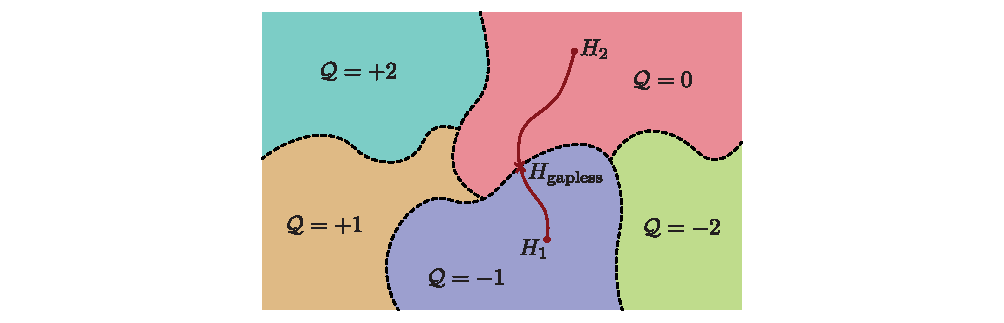
\includegraphics{introduction/figures/chern_classes.pdf}
    \caption[Illustration of the space of all non-interacting Hamiltonians, classified by their Chern numbers.]{
        The space of all Hamiltonians can be divided into a set of Chern classes defined by the bands' Chern numbers (only one band's Chern number is shown in this illustration). Adiabatically transforming from one Hamiltonian $H_1$ to another $H_2$ in a different Chern class, one necessarily crosses a point where the Hamiltonian becomes gapless.
    } 
    \label{fig:chern_classes}
\end{figure}

Using these methods, it was now possible to associate a quantised Chern number to each energy level in the band structure of a material. As per the original motivation, the Chern number determined the contribution of each band to the Hall conductivity. However, one could also view these invariants as a remarkably universal framework for classifying Hamiltonians, since their quantised nature meant that a band's Chern number could not change under adiabatic deformation of the system without closing the band gap (at which point the band, and thus $Q$, would be ill-defined). Thus, two Hamiltonians with different Chern numbers sit in two different Chern classes, where it is not possible to deform one into the other without a gap closing. Of course, these invariants strictly only applied to systems with a notion of band structure, i.e.~for non-interacting systems with translational symmetry. Several proposals exist for extending these invariants to interacting or disordered materials, most notably the construction of a local Chern marker \cite{kitaev_anyons_2006, markov_local_2021, loring_guide_2019, bianco_mapping_2011} which we shall discuss in Chapter \ref{chap:local_markers}. The simplest extension can be found by noting that the topological class of a Hamiltonian can only change with a closing of the band gap. Thus, as long as a general quantum system has a gapped ground state, and can (without closing this gap) be adiabatically connected to a Hamiltonian with well-defined Chern number, then the two systems are considered to have the same Chern numbers \cite{varney_topological_2011}. Thus, we see that, in analogy with the case of RG and universality discussed in the previous section, the Chern classification describes a set of physical properties that are deeply ambivalent to the microscopics of a model. Any changes to the system that do not close the band gap will have no effect on the Chern class or the Hall conductivity.

\section{Magnetism, Frustration and Fractionalisation}\label{sec:lattice_specific}

Let us now turn our attention to the opposite case to that discussed in \textsection\ref{sec:universality}, to systems whose properties are extremely sensitive to the microscopic arrangement of the material. One of the simplest examples can be found in the study of magnetism, by considering the Heisenberg model of interacting spins. We shall work with a toy model on an arbitrary lattice, consisting of a set of sites at positions $ \textbf{x}_j $ and a set of edges $e_{jk}$ that connect nearest-neighbour vertices at $ \textbf{x}_j $ and $ \textbf{x}_k$. At each vertex we place a single spin-$S$ degree of freedom, which interact with one another according to the Hamiltonian,
\begin{align} \label{eqn:heisenberg_model}
    H = - J \sum_{\braket{jk}} \textbf{s}_j \cdot \textbf{s}_k,
\end{align}
where the sum is only taken over nearest-neighbour pairs of spins and $J$ determines the strength and sign of each bond's coupling. In the ferromagnetic (FM) regime ( $J > 0$) this Hamiltonian favours the alignment of neighbouring spins and the ground-state can be straightforwardly constructed for any lattice by simply choosing a direction, say $\hat {\textbf z}$ and aligning all spins in that direction. Each bond contributes a value $-JS^2$ to the ground state energy -- the lowest contribution possible -- so we consider all bonds fully satisfied. This phase is stable on any lattice, with any values of $J_{jk}>0$. Thus, the ferromagnetic case falls into the class of models described in the previous section -- an emergent phase that is largely insensitive to the details of the system. 

Now let us consider the antiferromagnetic (AFM) case ($J_{jk} < 0$). Here neighbouring spins want to anti-align. On a bipartite lattice -- where all sites can be divided into two sublattices, $A$ and $B$, and a spin on an $A$-site is only adjacent to $B$-sites and vice-versa -- a similar ground state can be constructed. Choosing a direction, we can set all spins on the $A$ sublattice to point along this direction and all spins on the $B$ sublattice to point in the opposite direction. In the classical case ($S\gg 1$), this gives us the ground state, and all bonds are maximally satisfied, contributing $-|J_{jk}|S^2$ to the ground-state energy. In a quantum system, this antiferromagnetic alignment is typically a good approximation to the true long-range ordered Ne\'el state, which is generally dressed with additional correlations. However, on any lattice with odd-length cycles -- e.g.~a lattice containing triangles, pentagons etc.~-- this picture is dramatically altered. Now it is no longer possible to construct a N\'eel-ordered state since the system lacks sublattice symmetry. Rather, the ground state of the system will depend strongly on the geometry of the lattice \cite{richter_quantum_2004}. For example, after years of debate the consensus is that the triangular lattice forms a 120$^\circ$ ordered state \cite{huse_simple_1988,singh_three_1992,white_neel_2007}, shown in Fig.~\ref{fig:lattice_order_examples}b. On the star lattice, the ground state resists classical ordering altogether, forming a valence bond solid \cite{richter_absence_2004,choy_classification_2009,yang_competing_2010, jahromi_spin-frac12_2018,jahromi_infinite_2018,ran_emergent_2018}, shown in Fig.~\ref{fig:lattice_order_examples}c, where spins are strongly anti-correlated on the inter-triangle bonds, close to a singlet state, $\ket s = ( \ket{\uparrow\downarrow} - \ket{\downarrow\uparrow})/\sqrt 2$, and much more weakly correlated on the intra-triangle bonds.
\begin{figure}
    \centering
    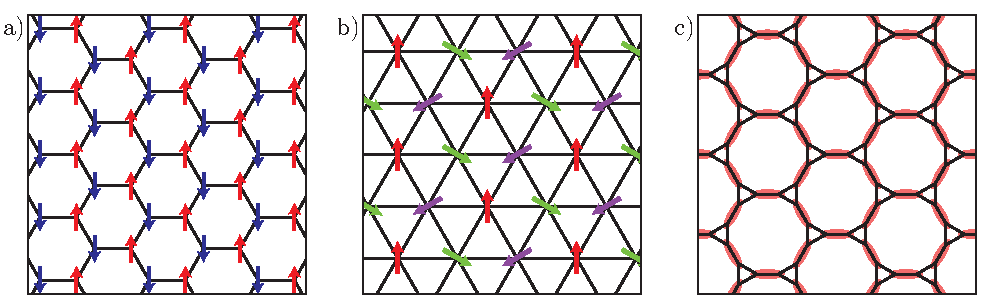
\includegraphics{introduction/figures/lattice_order_examples.pdf}
    \caption[Ground state of the spin-$\frac 12$ Heisenberg model on the honeycomb, triangular and star lattice.]{
        The ground state of the spin-$\frac 12$ antiferromagnetic Heisenberg model on three example lattices.
        \textbf{(a)}~The honeycomb lattice is bipartite, so the ground state is N\'eel ordered.
        \textbf{(b)}~On the triangular lattice the ground state is a three site 120$^\circ$ magnetically ordered phase. Here the spins are arranged such that the sum of the spins around each triangle always vanishes.
        \textbf{(c)}~On the star lattice, the system forms a valence bond solid, with spin singlets on the inter-triangle bonds, indicated by the red ellipses. 
    } 
    \label{fig:lattice_order_examples}
\end{figure}

As a rule of thumb, the magnetic properties of an antiferromagnetic material are most strongly influenced by two broad features of the lattice. The first is coordination number. In small-$S$ systems, lattices with low coordination numbers favour strong quantum fluctuations, reducing the likelihood of forming a classically-ordered ground state \cite{richter_quantum_2004}. The second property is frustration, and describes the extent to which the system is unable to simultaneously satisfy all bonds in the Hamiltonian, leading to a ground state energy that is higher than that in an equivalent unfrustrated system. In the example above, the triangle lattice is highly frustrated, but with a large coordination number, so forms a classical frustrated order. In the star lattice, the combination of low coordination number and frustration leads to the non-classical ground state. 

\subsection{Classical Frustration}

To better understand the role of frustration, let us consider the classical case, neglecting quantum fluctuations altogether. Our discussion will largely draw from the references \cite{ramirez_strongly_1994,moessner_magnets_2001,chalker_geometrically_2011}. In the large spin limit ($S\gg1$) the quantum spins, generally described in operator form and defined by their spin algebra, are well-approximated by a classical $d$-dimensional vector of fixed length $S$, where $d$ (generally $\leq 3$) defines the number of spin components. Let us set $J = -1$ and consider a cluster of $n$ fully interacting spins. The Hamiltonian of the cluster is given by
\begin{align}
    H_{Cl} = \frac 12 \sum_{jk} \textbf s_j \cdot \textbf s_k.
\end{align}
Constructing the total spin operator $\textbf S = \sum_{j}\textbf s_j$, this Hamiltonian can be rewritten as
\begin{align} \label{eqn:total_spin_trick}
    H_{Cl} = \frac 12 \left (
        |\textbf S|^2 - n S^2,
        \right )
\end{align}
where the constant terms come from the fact that $\textbf s_j \cdot \textbf s_j = S^2$. Thus, we see that the ground state corresponds to any arrangement with total spin $\textbf S = 0$, and has energy 
\begin{align}
    \egs = -nS^2/2.
\end{align}
This is in contrast with the unfrustrated energy that the system would have if all bonds were satisfied, given by 
\begin{align}E_{\textup{u.f.}} = - n!S^2/2,
\end{align}
where $n!/2$ is the number of bonds in a cluster of $n$ spins. The difference between the true ground state energy $\egs$ and the unfrustrated ground state energy $E_{\textup{u.f.}}$ can give a rough measure of the degree of frustration in the lattice \cite{kobe_frustration_1995}.

\begin{figure}
    \centering
    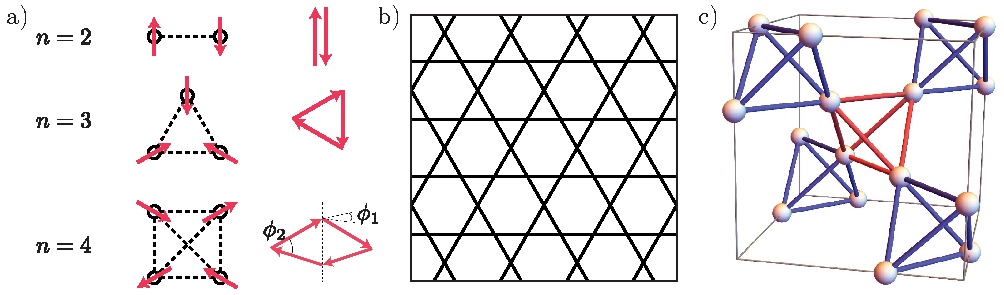
\includegraphics{introduction/figures/frustrated_intro.pdf}
    \caption[Ground state configuration for three clusters of $n$-spins, kagome lattice and pyrochlore lattice.]{
        \textbf{(a)}~Three clusters of $n \in \{2...4\}$ spins, showing a ground state configuration of spins. In the $n=2$ and $3$ case, there is a single unique configuration (up to global reflection and rotations), whereas for $n=4$ there are two independent degrees of freedom, marked with $\phi_m$ leading to an extremely degenerate ground state.  
        \textbf{(b)}~A section of kagome lattice, formed by vertex-sharing triangles. 
        \textbf{(b)}~A section of pyrochlore lattice, formed by vertex-sharing tetrahedra. \textit{ Figure reproduced from Theory of Quantum Matter Unit, OIST} 
        } 
    \label{fig:frustrated_simplex}
\end{figure}
Not only does frustration cause the ground state energy to be higher than one might expect based on the coupling strength, but it can also lead to systems with \textit{extensive ground state degeneracy}\footnote{Note that not all frustrated systems have degenerate ground states, for example the $120^\circ$ order found on the triangular lattice is non-degenerate.}. To see how this arises, let us count the number of ways to arrange the spins into an $\textbf S = 0$ state. For $n=2$ or $3$, ignoring overall rotations and reflections, there is one unique way. However, for $n=4$ we have two continuous degrees of freedom, shown in Fig.~\ref{fig:frustrated_simplex}a. 

Now, let us consider a generic corner-sharing lattice composed of $N_c$ clusters, for example the kagome lattice with $n=3$ shown in Fig.~\ref{fig:frustrated_simplex}b, or the pyrochlore lattice with $n=4$, shown in Fig.~\ref{fig:frustrated_simplex}c. The Hamiltonian can again be decomposed into a sum of the total spin for each interacting cluster, this time ignoring the constant terms,
\begin{align}
    H = \sum_{n_c}^{N_c} |\textbf S_{n_c}| - \textit{constant}.
\end{align}
Again, the ground state is found by setting the total spin through each cluster to zero. The ground state degeneracy can be estimated by noting that of each spin contributes $d-1$ degrees of freedom, each cluster contributes $d$ constraints. Thus, one naively expects the ground state to have
\begin{align}
    D = \frac{N_c}{2} 
    \left (
        n(d-1) - 2d
    \right )
\end{align}
remaining degrees of freedom, where the factor of a half comes from the fact that each spin forms part of two clusters. According to this, the Kagome lattice ($n=3$) has no remaining degrees of freedom, but the pyrochlore lattice has an extensive ground state degeneracy, with each tetrahedron contributing one parameter that can be freely adjusted while remaining in the ground state. In fact, this guess is usually an underestimate, since it does not take into account the fact that the constraints of adjacent plaquettes are not completely independent. For example, the kagome lattice ground state can, in certain ground states, be rotated locally around certain hexagons as shown in Fig.~\ref{fig:kagome_rot}a, leading to a $D = N_c/9$ remaining unconstrained degrees of freedom \cite{ritchey_spin_1993,chalker_hidden_1992}. In general, such remaining degrees of freedom are highly specific to the geometry of the lattice. For example, adding in an extra site to the kagome as shown in Fig.~\ref{fig:kagome_rot}b has the effect of combining three regions, which must now be rotated together, effectively removing two degrees of freedom, despite the fact that the frustration as measured by comparing $\egs$ and $E_{\textup{u.f.}}$ has not changed. 

\begin{figure}
    \centering
    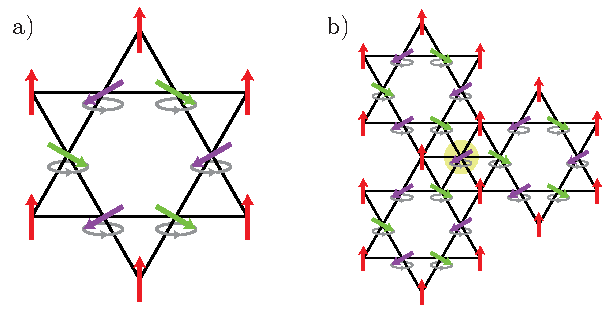
\includegraphics{introduction/figures/kagome_rot.pdf}
    \caption[Ground state degeneracy in the Kagome antiferromagnet.]{
        \textbf{(a)}~On the Kagome lattice, the spin arrangement shown can undergo a simultaneous rotation of the purple and green spins without leaving the ground state.
        \textbf{(b)}~Modifying the lattice, for example by adding the central purple spin, triples the size of the regions that must be rotated together, removing two degrees of freedom. 
        } 
    \label{fig:kagome_rot}
\end{figure}

\subsection{The Classical Kitaev's Honeycomb Model}

Thus far, we have only discussed so-called \textit{geometrical} frustration, where the inability of the system to satisfy all couplings is driven by the geometry of the lattice -- usually the presence of odd cycles. However, frustration can also be introduced through the engineering of competing interactions on lattices that would otherwise not be considered frustrated, a type of frustration we shall refer to as \textit{exchange} frustration. Here we shall present one such model, the Kitaev honeycomb model \cite{kitaev_anyons_2006}. As the name suggests, the model is constructed on a honeycomb lattice, with a spin placed at each vertex. In the original formulation, Kitaev proposed (and solved) the quantum spin-$\frac 12$ model. In Chapter \ref{chap:amorphous_kitaev} we shall discuss in detail the method that he used for solving this model, as well as generalising it to arbitrary lattices. Thus, here let us start by considering the large-$S$, classical Kitaev model. This has been extensively studied \cite{baskaran_spin_2008,samarkoon_comprehensive_2017,rousochatzakis_quantum_2018,ma_z2_2023}.  Here we focus on the first part of the classical story, finding the ground state and discussing its degeneracy. 

To construct the Hamiltonian, we must assign a label $\alpha \in \{x,y,z\}$ to each bond on the honeycomb, such that every vertex connects to one bond of each type, shown in Fig.~\ref{fig:kitaev_intro}. The Hamiltonian is given by,
\begin{align} \label{eqn:classical_kitaev_hamiltonian}
    H =  
    - J^x \sum_{\braket{jk}_x} s_j^x s_k^x
    - J^y \sum_{\braket{jk}_y} s_j^y s_k^y
    - J^z \sum_{\braket{jk}_z} s_j^z s_k^z,
\end{align}
where $\braket{jk}_\alpha$ indicates a bond of type $\alpha$. Let us work at the so-called isotropic point, found by setting all $J^\alpha = +1$, ensuring that each coupling is ferromagnetic.\footnote{We could equivalently use $J = -1$, since this Hamiltonian can be transformed back to the $J=+1$ case by reversing the orientation of every spin on the $B$ sublattice.}

\begin{figure}
    \centering
    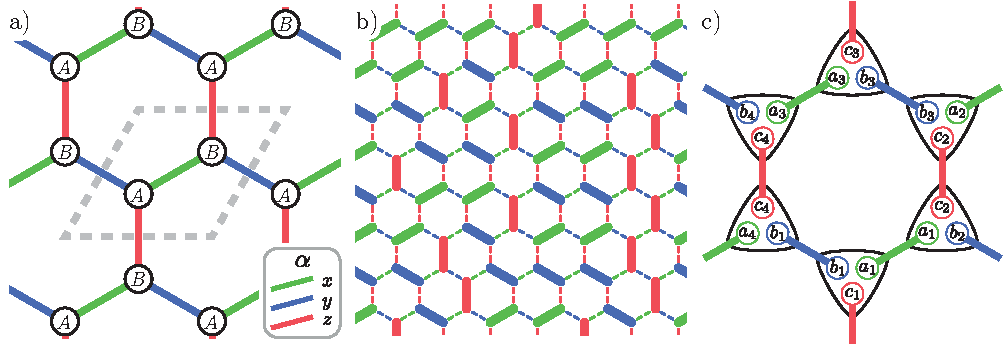
\includegraphics{introduction/figures/kitaev_intro.pdf}
    \caption[Bond colouring for the honeycomb Kitaev model and classical ground state configuration.]{
        \textbf{(a)}~The honeycomb lattice on which the Kitaev model is constructed. Bond labelling is indicated by colour, and the unit cell is shown by the dashed grey rhombus.
        \textbf{(b)}~An example Cartesian state, where the adjacent spins on every highlighted bond are fully aligned in the direction corresponding to that bond's label, forming a dimerisation of the full lattice.
        \textbf{(c)}~A parametrisation of the general classical Kitaev ground state, formed by setting the $\alpha$-component of neighbouring spins on each side of an $\alpha$-bond to be equal to one another.
        } 
    \label{fig:kitaev_intro}
\end{figure}
We wish to find the lowest energy state that satisfies $\textbf s \cdot \textbf s  = S^2$. Thus, let us enforce this total spin condition by adding a Lagrange multiplier to the Hamiltonian,
\begin{align}
    H_{\lambda} =     
    - \sum_{\braket{jk}_\alpha} s^\alpha_j s^\alpha_k
    - \frac 12\sum_j \lambda_j ( \textbf s \cdot \textbf s - S^2)
\end{align}
Taking a derivative w.r.t.~the components of the two spins around an $\alpha$-bond, $s^\alpha_j$ and $s^\alpha_k$, we arrive at the following conditions
\begin{align}
    s^\alpha_k = \lambda_j s^\alpha_j, \label{eqn:a_j_lambda}
    \\
    s^\alpha_j = \lambda_k s^\alpha_k. \label{eqn:a_k_lambda}
\end{align}
Thus, we may use relation
\begin{align}
    s^x_js^x_k = \lambda_j s^{\alpha2}_j + = \lambda_k s^{\alpha2}_k,
\end{align} 
to re-express the Hamiltonian in two equivalent forms
\begin{align} \label{eqn:H_two_ways}
    H =
    -S^2\sum_{j \in A} \lambda_j,
     = 
    -S^2\sum_{j \in B} \lambda_j,
\end{align}
where we used the  condition $\textbf s \cdot \textbf s = S^2$. Now all that remains is to find the values of $\lambda_j$. For a given site, at least one of the three spin components at that site must be nonzero. Thus, for this pair we may substitute Eqns.~\ref{eqn:a_j_lambda} and \ref{eqn:a_k_lambda} into one another to obtain the relation, $\lambda_j \lambda_k = 1$. Since the lattice is bipartite, extrapolating this relation implies that $\lambda_j = \lambda_A $ must be constant across all $A$ sites, with the same relation holding for $B$ sites. Furthermore, from Eqn.~\ref{eqn:H_two_ways} we see that $\lambda_A = \lambda_B$. Thus, the lowest energy is found by setting all $\lambda = +1$,
\begin{align}
    \egs = -\frac 12 S^2 N_s,
\end{align}
with $N_s$ being the number of sites in the system. Thus, the ground states may now be constructed, since we must simply choose a configuration that saturates the lower bound for the energy, as well as the conditions $s^\alpha_j = s^\alpha_k$ for each pair of sites that share an $\alpha$-bond. The simplest ground states, which we refer to as the Cartesian states, are found by leaving only one of the three components of $\textbf s_j$ nonzero on each site. To be a valid ground state, every site must be paired up with a neighbour, forming a dimerisation where the two spins around a dimer on an $\alpha$-bond are completely aligned in the $\alpha$ direction. An example is shown in Fig.~\ref{fig:kitaev_intro}b. Thus, the degeneracy of the Cartesian states can be found by counting the number of dimerisations, which scales with $1.381^{N_s/2}$ \cite{wannier_antiferromagnetism_1950, kasteleyn_dimer_1963}. However, since each dimer has two directions it can align in, the degeneracy is
\begin{align}
    n_{\textup{Cart.}} = 1.662^{N_s}.
\end{align}
However, the Cartesian states are not disconnected from one another, since it is possible to transform any Cartesian state into any other smoothly without leaving the ground state. This can be done by noting that any state that satisfies $s^\alpha_j = s^\alpha_k$ on every bond is also in the ground state. Thus, a general ground state may be constructed by choosing one parameter for each bond, we shall use $a$ on $x$-bonds, $b$ on $y$-bonds and $c$ on $z$-bonds, and assigning the components of $\textbf s$ according to the three bond variables on each site, as shown in Fig.~\ref{fig:kitaev_intro}c. Provided that the bond parameters on any site satisfy $a^2 + b^2 + c^2 = S^2$, a state of this form automatically saturates the lower bound for the energy. The ground state degeneracy can then be approximated by noticing that this ansatz has one degree of freedom for every bond, and one constraint -- the total spin $S$ -- for every site. Since each site connects to 3 bonds, this leaves $D = N_s/2$ remaining degrees of freedom.

\subsection{A Quantum Spin Liquid}

So far we have defined a notion of magnetic frustration, and shown how it can arise both as a consequence of lattice geometry or, as in the Kitaev case, due to the presence of competing interactions. In a classical system, often the consequence of frustration is the creation of an extensive number of degenerate ground states. This allows classically frustrated systems to avoid magnetically ordering at low temperatures, since even a small amount of thermal energy is sufficient for the system to freely explore these degenerate states. Indeed, one of the most robust signatures of frustration is that -- in contrast to unfrustrated ferro- and antiferromagnets, which undergo a spin-ordering (or freezing) transition at a temperature determined by the microscopic coupling strength \cite{simon_oxford_2013} --  frustrated magnets tend to remain paramagnetic (or liquid) down to far lower temperatures than their coupling strength would suggest \cite{chalker_geometrically_2011,mugiraneza_tutorial_2022}. In fact in some systems, notably in the case of spin ice \cite{castelnovo_magnetic_2008,castelnovo_spin_2012,udagawa_spin_2021}, the system does not undergo an ordering transition at any temperature. Such materials are collectively known as classical spin liquids, in reference to the unusually low temperatures to which these paramagnetic (liquid) phases persist. 

However, thermodynamics is not the only mechanism by which fluctuations arise in nature. When the spin in a frustrated magnet is small (that is, close to $S = \frac 12$), quantum fluctuations can play a significant role, allowing the spins to resist ordering even at zero temperature. Furthermore, the consequences of quantum fluctuations can be drastically different from the classical case, since a quantum system is able to form coherent superpositions of these degenerate classical states. Thus, it is possible for the ground-state degeneracy of a classical spin liquid to be broken in the equivalent quantum system, which finds a lower-energy \textit{quantum spin liquid} (QSL) ground state. Since a QSL state arises necessarily as a consequence of quantum effects, they are highly entangled states of matter which provide a rich context for finding exotic phenomena with no classical analogue. Although no formally accepted definition exists, the consensus is that to qualify as a QSL a phase of matter must exhibit some combination of two related emergent properties: fractionalised excitations and an emergent gauge field \cite{knolle_field_2019,savary_quantum_2017}.

In a fractionalised system, the quasiparticles carry a fraction of the properties of the constituent particles in the material. The most famous example of this phenomenon is the fractional quantum Hall effect \cite{laughlin_nobel_1999}, where the quasiparticles carry a fraction of the charge (and a fraction of the exchange statistics) of the electron. However, the last 30 years of research has revealed an astonishing number of ways that fractionalised particles can appear. For example, in classical spin ice, the natural dipolar spin-flip excitations split into pairs of magnetic monopoles, and as we shall see in the following discussion (and in detail in Chapter \ref{chap:amorphous_kitaev}) excitations take the form of Majorana fermions in the Kitaev model. Of course, even in a fractionalised material, one must respect the conservation laws implied by the original, unfractionalised constituents. That is, quantities such as the total charge, or the total magnetic moment of the system are not allowed to take fractionalised values. In a quantum Hall system where quasiparticles have $\frac pq$ charge, we must ensure that the system always contains a multiple of $q$ such particles. Similarly, monopoles in spin ice must always be created and destroyed in pairs, else the system as a whole will have nonzero magnetic charge, which is forbidden in electromagnetism. This global constraint means that an effective description of the system must include an emergent gauge field, whose rose is to enforce this symmetry, encoding the constraint locally in the configuration of the field. 

Let us end this section by describing the exact solution to the spin-$\frac 12$, quantum Kitaev model and showing how it satisfies these two requirements. Note that this will largely be a qualitative discussion, and a careful derivation is presented in Chapter \ref{chap:amorphous_kitaev}. In the spin-$\frac 12$ version, we are no longer free to treat spins as a classical vector, and instead must express the Hamiltonian, Eqn.~\ref{eqn:classical_kitaev_hamiltonian}, in terms of the Pauli matrices that determine the spin algebra,
\begin{align}
    s_x \rightarrow \frac 12\sigma^x ,\qquad
    s_y \rightarrow \frac 12\sigma^y ,\qquad
    s_z \rightarrow \frac 12\sigma^z .
\end{align}
Discarding a global factor of $\frac 12$, the Kitaev Hamiltonian takes the form 
\begin{align}
    H = - \sum_{\braket{jk}_\alpha} J^\alpha \sigma^\alpha_j \sigma^\alpha_k.
\end{align}
To diagonalise this Hamiltonian, Kitaev transformed to an artificially enlarged Hilbert space by replacing each spin-half degree of freedom with four Majorana fermionic operators, labelled as $c, b^x, b^y$ and $b^z$ according to the transformation $\sigma^\alpha_j \rightarrow i c_j b^\alpha_j$. These operators are self-adjoint, and obey fermionic anti-commutation relations,
\begin{align}
    c^\dag &= c,\\
    \{c_j, c_k\} &= \delta_{jk}
\end{align}
At each site, these four Majoranas correspond to two fermionic operators, since one can combine a pair of Majoranas, $c_j$ and $c_k$, to create an operator $f$ that obeys standard fermionic commutation relations, $f = \frac 12 (c_j + i c_k)$, with $\{f_j ,f_k^\dag\} = \delta_{jk}$. After performing this transformation, Kitaev showed that the $b$-type Majoranas were essentially static, where the two $b^\alpha$ operators adjacent to each $\alpha$-bond could be paired up as a conserved operator $\hat u_{jk} = ib^\alpha_j b^\alpha_k$. Because each site connected to only one bond of each type, each $\hat u_{jk}$ operator also showed up only once, and commute with each other as well as the Hamiltonian. This meant that they could be treated as a conserved quantity, and replaced in $H$ with their eigenvalues, $\hat u_{jk} \rightarrow \ujk = \pm 1$, resulting in a final Majorana Hamiltonian of the form,
\begin{align}
    H = \sum_{\braket{jk}_\alpha} J^\alpha \ujk c_j c_k.
\end{align}

We started with a system of interacting spins, however the Hamiltonian here constitutes a very different description of the model. Here, the spins have been transformed into two very different decrees of freedom, coupled to one another. In the $c_j$ operators we have a set of $N_s$ 

Thus, we see that the two Majorana fermions can be viewed as a fractionalised quasiparticle, corresponding to half a fermionic degree of freedom. 



% \begin{align}
%     H = J^\alpha \sum_{\braket{jk}_\alpha} (i b^\alpha_j b^\alpha_k) i c_j c_k.
% \end{align}

\section{Thesis Outline}

Thus far we have discussed examples of physical phenomena, namely the notion of universality and the quantum Hall effect  
\printbibliography[heading=subbibintoc]

\chapter{Chern Number, Topological Insulators and Local Markers}
Paragraph introducing the topics covered in this section. Points to hit:
\begin{itemize}
    \item 
\end{itemize}


% The aim of the first half of this thesis is to understand how the Chern number -- which is well-defined only for non-interacting quantum systems with translational symmetry -- can be extended to disordered materials. 

% There are three parts, first we introduce the concepts of Berry phase and Chern number, discussing the ways that they can be used to classify non-interacting quantum systems with no symmetries. Next we define the Qi-Wu-Zhang model, which provides a simple example of a Chern insulator on a square lattice. 

\section{Abelian Berry Phase and the Chern Number} \label{sec:Abelian Berry Phase and the Chern Number}

In this section we present a careful discussion of Berry's phase, Berry curvature and the Chern number \cite{berry_quantal_1984,avron_homotopy_1983}, showing how these quantities may be calculated form the band structure of a general non-interacting insulator. There are two cases to discuss: for a finite system the Brillouin zone constitutes a discrete lattice of states. Thus, in \textsection\ref{sec:discrete_berry}, we show that Berry phase can be understood as the relative phase between adjacent states, and that Berry flux is defined on the plaquettes of the lattice. In \textsection\ref{sec:continuous_berry} we consider the case of an infinite system. There the Brillouin zone is a continuous manifold and the band structure defines a mapping from this manifold to the Hilbert space of periodic states. In this case, Berry's phase is a geometric property of this smooth mapping. In both cases, we derive the form of the Chern number and justify its quantisation. Finally, in \textsection\ref{sec:an_example} we provide an example -- that of a two level system -- where the Berry flux can be understood straightforwardly in terms of the flux emitted by a monopole, allowing us to present a simple visual argument for the quantisation of the Chern number. Our discussion will largely follow \cite{asboth_berry_2016,resta_geometry_2020}.

\subsection{A Discrete Brillouin Zone} \label{sec:discrete_berry}

In quantum mechanics a state is defined as an equivalence class of vectors, where two states that differ only by a complex phase are considered physically equivalent,
\begin{align}
    \ket{\psi} \sim e^{-i\alpha}\ket{\psi}.
\end{align}
Thus, we have a redundancy built into our description of physics. This means that one can define a gauge transformation -- multiplying a state with a complex phase, a $U(1)$ gauge -- that is guaranteed not to affect the state in any measurable way. Any derived quantity must be invariant under gauge transformations to qualify as a physical observable.

Now, let us consider an arbitrary set of states in the same Hilbert space, $\{ \ket{\psi_j}\}$. Analogous to the `global' gauge transformation presented above, we may define a `local' gauge transformation here, where we apply a different phase to each individual state,
\begin{align}
    \ket{\psi_j} \rightarrow e^{-i\alpha_j}\ket{\psi_j}.
\end{align}
Again, the physical meaning of each state is unaffected, so all observable quantities must be invariant under this transformation. Thus, one might wonder whether any \textit{phase-like} quantity calculated from these states can have a physical meaning. For example, the relative phase between state $j$ and $k$, $\gamma_{j,k}$ can be defined as
\begin{align}
    e^{-i\gamma_{j,k}} = \frac{\braket{\psi_j|\psi_k}}{|\braket{\psi_j|\psi_k}|}.
\end{align}
Clearly this quantity is invariant under a global gauge transformation, however it is not invariant under a local transformation, changing according to
\begin{align}
    e^{-i\gamma_{j,k}} \rightarrow e^{-i(\gamma_{j,k}+\alpha_j - \alpha_k)},
\end{align}
and so cannot be a physical observable. In order to construct a gauge-invariant object, let's pick a set of $n$ ($\geq 3$) states $\ket{\psi_j}$ and arrange them in a loop.
\begin{center}
    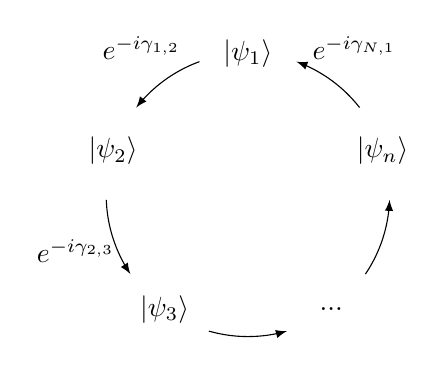
\begin{tikzpicture}

\def  \angoff {20}
\def \picsize {1.8}
\def \edistance {0.5}
\def \anground {72}

\draw [-latex,domain = \angoff:\anground-\angoff] plot ({\picsize * cos (\x + 90)}, {\picsize * sin (\x + 90)});
\draw [-latex,domain = \angoff:\anground-\angoff] plot ({\picsize * cos (\x + 90+\anground)}, {\picsize * sin (\x + 90+\anground)});
\draw [-latex,domain = \angoff:\anground-\angoff] plot ({\picsize * cos (\x + 90+2*\anground)}, {\picsize * sin (\x + 90+2*\anground)});
\draw [-latex,domain = \angoff:\anground-\angoff] plot ({\picsize * cos (\x + 90+3*\anground)}, {\picsize * sin (\x + 90+3*\anground)});
\draw [-latex,domain = \angoff:\anground-\angoff] plot ({\picsize * cos (\x + 90+4*\anground)}, {\picsize * sin (\x + 90+4*\anground)});

\draw node at (90:\picsize) {$\ket{\psi_1}$};
\draw node at (90+\anground:\picsize) {$\ket{\psi_2}$};
\draw node at (90+2*\anground:\picsize) {$\ket{\psi_3}$};
\draw node at (90+3*\anground:\picsize) {$...$};
\draw node at (90+4*\anground:\picsize) {$\ket{\psi_n}$};

\draw node at (90+0.5*\anground:\picsize+\edistance) {$e^{-i \gamma_{1,2}}$};
\draw node at (90+1.5*\anground:\picsize+\edistance) {$e^{-i \gamma_{2,3}}$};
\draw node at (90+4.5*\anground:\picsize+\edistance) {$e^{-i \gamma_{N,1}}$};

\end{tikzpicture}
\end{center}
We can now define a new quantity, the Berry phase, as
\begin{align}
    e^{-i \gamma_{B}} = \frac{\braket{\psi_1|\psi_2}\braket{\psi_2|\psi_3}...\braket{\psi_N|\psi_1}}{|\braket{\psi_1|\psi_2}\braket{\psi_2|\psi_3}...\braket{\psi_N|\psi_1}|}
\end{align}
Another way of writing this would be
\begin{align}  
    \gamma_{B} = -\arg \tr 
    \left [ \hat\psi_{1} \hat\psi_{2} 
    \, ... \,
    \hat\psi_{N} \right ],
\end{align}
where the trace is over the whole system, and $\hat \psi$ is shorthand for the density operator
\begin{align}
    \hat \psi_{i} = \ket{\psi_{i}}\bra{\psi_{i}}.
\end{align}
This quantity is clearly gauge-invariant, since any phase applied to a state $\ket{\psi_m}$ will show up twice, once from $\braket{\psi_m|\psi_{m+1}}$ and once from $\braket{\psi_{m-1}|\psi_{m}}$. The phase will have opposite sign in each of these expressions, so they cancel out. Furthermore, we can see that the Berry phase around a loop is simply the sum of all the relative phases around that loop modulo $2\pi$.
\begin{align}\label{eqn:discrete_berry_sum}
	\gamma_B = \sum_{n=1}^N \gamma_{n,n+1} \mod 2\pi
\end{align}


\subsubsection{Berry Flux}

Now suppose that we have a large number of states arranged in a 2D grid. These states  $\ket{\psi_{\textbf k}}$ are labelled with a pair of indices $k_x$ and $k_y$. In general, this parameter $\textbf k$ will refer to the crystal momentum, however the construction is equally valid for any other parameter that defines a 2D grid of quantum states, shown in Fig.~\ref{fig:berry_grid}.

\begin{figure}
    \begin{center}
        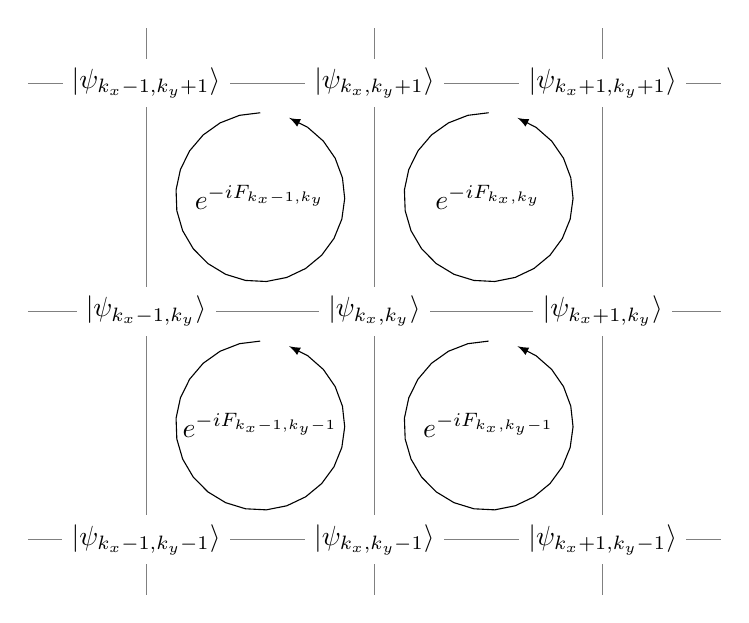
\begin{tikzpicture}

\def \gridsize{2.9}

\draw[step=\gridsize cm, help lines] (-\gridsize-1.5,-\gridsize-0.7) grid (\gridsize+1.5,\gridsize+0.7);
\draw node [fill= white] at (0,0) {$\ket{\psi_{k_x,k_y}}$};
\draw node [fill= white] at (\gridsize,0) {$\ket{\psi_{k_x+1,k_y}}$};
\draw node [fill= white] at (\gridsize,\gridsize) {$\ket{\psi_{k_x+1,k_y+1}}$};
\draw node [fill= white] at (0,\gridsize) {$\ket{\psi_{k_x,k_y+1}}$};
\draw node [fill= white] at (-\gridsize,0) {$\ket{\psi_{k_x-1,k_y}}$};
\draw node [fill= white] at (0,-\gridsize) {$\ket{\psi_{k_x,k_y-1}}$};
\draw node [fill= white] at (-\gridsize,-\gridsize) {$\ket{\psi_{k_x-1,k_y-1}}$};
\draw node [fill= white] at (\gridsize,-\gridsize) {$\ket{\psi_{k_x+1,k_y-1}}$};
\draw node [fill= white] at (-\gridsize,\gridsize) {$\ket{\psi_{k_x-1,k_y+1}}$};

\draw [-latex, domain = 0:340] plot ({0.37 *\gridsize* cos (\x + 90) + 0.5 * \gridsize }, {0.37 *\gridsize* sin (\x + 90) + 0.5 *\gridsize });
\draw [-latex, domain = 0:340] plot ({0.37 *\gridsize* cos (\x + 90) - 0.5 * \gridsize }, {0.37 *\gridsize* sin (\x + 90) + 0.5 *\gridsize });
\draw [-latex, domain = 0:340] plot ({0.37 *\gridsize* cos (\x + 90) + 0.5 * \gridsize }, {0.37 *\gridsize* sin (\x + 90) - 0.5 *\gridsize });
\draw [-latex, domain = 0:340] plot ({0.37 *\gridsize* cos (\x + 90) - 0.5 * \gridsize }, {0.37 *\gridsize* sin (\x + 90) - 0.5 *\gridsize });

\draw node at (0.5*\gridsize, 0.5*\gridsize) {$e^{-i F_{k_x,k_y}}$};
\draw node at (0.5*\gridsize, -0.5*\gridsize) {$e^{-i F_{k_x,k_y-1}}$};
\draw node at (-0.5*\gridsize, 0.5*\gridsize) {$e^{-i F_{k_x-1,k_y}}$};
\draw node at (-0.5*\gridsize, -0.5*\gridsize) {$e^{-i F_{k_x-1,k_y-1}}$};

\end{tikzpicture}
    \caption[A grid of states parametrised by a discrete parameter. ]{A grid of states parametrised by the discrete variables $\textbf k$, given by $\ket{\psi_{k_x,k_y}}$. For each plaquette, the Berry phase is calculated by taking the inner products of the states going counterclockwise around the loop.}
    \label{fig:berry_grid}
    \end{center}
\end{figure}%

We introduce a new quantity called the Berry flux, defined as the Berry phase around a plaquette on the grid,
\begin{align}\label{eqn:berry_flux}
    F_{\textbf k} =  
    - \arg \tr \left [ 
        \hat \psi_{k_x,k_y}
        \hat \psi_{k_x+1,k_y}
        \hat \psi_{k_x+1,k_y+1}
        \hat \psi_{k_x,k_y+1} 
        \right ].
\end{align}
$F_{\textbf k}$ is just the sum (mod $2\pi$) of the relative phases along each edge of the plaquette starting at point $\textbf k$. Thus, the Berry phase around some arbitrary loop can be written as a sum of the Berry flux for all plaquettes encircled by the loop. In this sum, the phase along any internal edge appears with opposite sign in the values of $F_{\textbf k}$ for the two adjacent plaquettes, leaving only the phase along the boundary,
\begin{align} \label{eqn:berry_sum_discrete}
    \exp 
    \bigg [
        -i \sum_{\substack{\textup{inside} \\ \textup{region}}}F
    \bigg ] 
    = \exp \bigg [ 
        -i\sum_{\textup{boundary}} \gamma
    \bigg ]
\end{align}
This resembles Stokes' law, however there is a subtlety worth mentioning. All we have required is that the complex exponential of each sum is the same. This does \textbf{not} mean that the sum of the Berry flux inside a region is equal to the sum of relative phases around the boundary, since they are allowed to differ by an arbitrary multiple of $2\pi$.


\subsubsection{Chern Number} \label{sec:discrete_chern}
Now let's assume that our grid of $\textbf k$ points has periodic boundaries -- as is the case for states on the Brillouin zone -- with $1\leq k_x \leq N_x$ and $1 \leq k_y \leq N_y$. The lattice is a discretisation of the torus -- a closed manifold. Thus, let us ask what the total flux through the whole manifold is. Following the argument of Eqn.~\ref{eqn:berry_sum_discrete}, the total Berry flux must satisfy 
\begin{align}\label{torus_sum}
    \prod_{k_x=1}^{N_x}\prod_{k_y=1}^{N_y}e^{-i F_{k_x,k_y}} = 1,
\end{align}
because every edge in this sum is an internal edge, and thus they cancel out. As before, this does not mean that the sum of all Berry fluxes in the system vanishes, rather the sum must be a multiple of $2\pi$. Thus let us define this multiple as the Chern number, $\mathcal Q$,
\begin{align}\label{eqn:discrete_chern_number}
    \mathcal Q = \frac{1}{2\pi} \sum_{k_x,k_y}F_{k_x,k_y}.
\end{align}
$\mathcal Q$ is necessarily restricted to integer values, since a non-integer value would contradict equation \ref{torus_sum}.

\subsection{Topology of a General Hamiltonian}\label{sec:continuous_berry}

Now let us consider the case of a smooth parameter space. We start by defining some arbitrary Hamiltonian $H(\textbf R)$, which depends on some smooth parameter $\textbf R \in \mathcal R$. For every value of $\textbf R$, the Hamiltonian has eigenstates $\ket{\psi_n (\textbf R)}$ with corresponding energies $\varepsilon_n$. As before, these eigenstates are only well-defined up to a global phase. Thus, let consider a single state $\ket{\psi(\textbf R)}$ and define a local gauge transformation, applying an $\textbf R$-dependent phase $\alpha(\textbf R)$ to all the states over this band.
\begin{align}
	\ket{\psi(\textbf R)} \rightarrow e^{-i\alpha(\textbf R)}\ket{\psi(\textbf R)}.
\end{align}
Before we continue, let us define a \textit{smooth gauge} as a choice of gauge that ensures that the $\textbf R$-derivative of a state, $\nabla_{\textbf R}\ket{\psi(\textbf R)}$ is always well-defined -- that is, $\alpha(\textbf R)$ does not change discontinuously. In general, it is not always possible to pick a gauge that is globally smooth over all of $\mathcal{R}$, however it \textit{is} always possible to pick a locally smooth gauge around the neighbourhood of a given point in $\mathcal{R}$.

In analogy to the relative phase in the previous section, let us quantify phase between a state at $\textbf R$ and a state that is infinitesimally displaced from it, at $\textbf R + d \textbf R$,
\begin{align}
    e^{-i\Delta\gamma} = \frac{\braket{\psi(\textbf R)|\psi(\textbf R+d\textbf R)}}{|\braket{\psi(\textbf R)|\psi(\textbf R+d\textbf R)}|}.
\end{align}
Taking the limit of small $d\textbf R$ we can express $\ket{\psi(\textbf R+d\textbf R)}$ to first order in $d\textbf R$ as
\begin{align}
    \ket{\psi(\textbf R+d\textbf R)} = \ket{\psi(\textbf R)} + d\textbf R \cdot \nabla_{\textbf R} \ket{\psi(\textbf R)}.
\end{align}
Which means that
\begin{align}
    \braket{\psi(\textbf R)|\psi(\textbf R+d\textbf R)} = 1 + \braket{\psi(\textbf R) | \nabla _{\textbf R}|\psi(\textbf R)}\cdot d\textbf R .
\end{align}
Now, noticing that $ \braket{\psi(\textbf R) | \nabla_{\textbf R} |\psi(\textbf R)}$ is pure imaginary, we can show that
\begin{align}\label{A_def}
    \Delta \gamma &= \textbf{A} \cdot d\textbf R, \\
    \textbf{A}(\textbf R)& = i
    \braket{\psi(\textbf R) | 
    \nabla_{\textbf R} |
    \psi(\textbf R)} . \label{eqn:cont_berry_connection}
\end{align}
The quantity multiplying $d\textbf R$ is the Berry connection $\textbf{A}(\textbf R)$. Like the relative phase in the previous section, it is not a gauge-invariant quantity. Under a gauge transformation it changes according to
\begin{align} \label{eqn:gauge}
    \textbf{A}(\textbf R) \rightarrow \textbf{A}(\textbf R) - \nabla _{\textbf R} \alpha(\textbf R)
\end{align}
Now let us suppose that we slowly transform our Hamiltonian around some closed path $\mathcal C$ in $\textbf R$-space and keep track of the phase picked up by a given state.\footnote{In \cite{berry_quantal_1984}, Berry originally proposed this transformation as an adiabatic process, where we modify the Hamiltonian extremely slowly, and many sources (e.g.~\cite{xiao_berry_2010}) propose the Berry phase in that framework. In that case, one has to do a little extra work to keep track of the energy-dependent phase that a state picks up $\sim e^{-i \varepsilon t}$ alongside the topological phase determined by $\textbf A$. Here we shall neglect this, only considering the \textit{instantaneous eigenstates} at different values of $\textbf R$. For a thorough explanation, see \cite{vanderbilt_berry_2018}.} In analogy with Eqn.~\ref{eqn:discrete_berry_sum}, the Berry connection allows us to calculate the total phase accumulated over this route, according to
\begin{align} \label{eqn:flux_loop}
    \gamma(\mathcal C) = \oint_{\mathcal C} \textbf{A} \cdot d\textbf R.
\end{align} 

\begin{figure}
    \begin{center}
     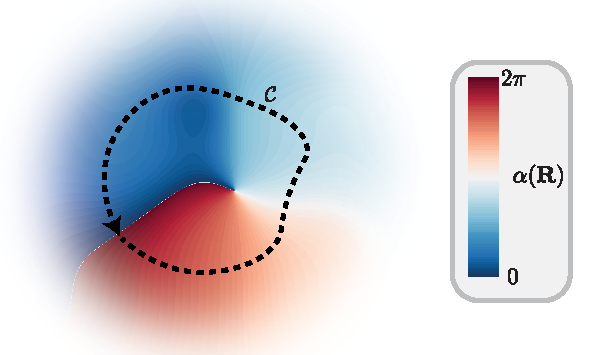
\includegraphics[]{local_markers_background/figures/branch cut.pdf}
    \caption[Colourmap of a local gauge transformation. ]{An example of a non-smooth gauge transformation designed to change the value of the Berry phase around the path $\mathcal C$ -- marked with a dashed line -- by an addition of $2\pi$. Only a small region of $\textbf R$-space is shown, with the local phase applied shown by the colourmap.}
    \label{fig:branch_cut}
    \end{center}
\end{figure}%
The exponential of the phase $e^{-i\gamma(\mathcal C)}$ around the loop \textit{is} gauge invariant, one can see this intuitively by realising that it is identical to the Berry phase from the discrete case, but in the limit where the discrete steps become arbitrarily close together. However, the Berry phase $\gamma(\mathcal C)$ itself is not strictly gauge invariant, since one can introduce a gauge transformation that creates a branch cut around the path $\mathcal C$. After traversing the whole path, the state at the end of the loop would have picked up a total phase $2\pi$, meaning that under a gauge transformation we can change the Berry phase according to 
\begin{align}
    \gamma (\mathcal C) \rightarrow \gamma (\mathcal C) + 
     2\pi n \textup{ for } n \in \mathbb Z.
\end{align}
An example of such a gauge transformation is shown in Fig.~\ref{fig:branch_cut}

\subsubsection{Berry Curvature}
Let us now define a quantity equivalent to the Berry flux from the previous discussion. Starting with Eqn.~\ref{eqn:flux_loop}, we use Stokes' theorem to transform it into a surface integral over a surface $\mathcal S$ bounded by the curve $\mathcal C$. We will consider the case for a two and three-dimensional parameter space $\mathcal R$, but of course this argument generalises to arbitrary dimensions.
\begin{align}
    \textup{In 2D: } & \gamma (\mathcal C) = \int_{\mathcal S} d^2R 
    \left ( 
        \partial_{x} A_{y}(\textbf R) - \partial_{y}A_{x}( \textbf R) 
    \right ) , \label{eqn:2d_berry_curvature} \\
    \textup{In 3D: } & \gamma (\mathcal C) = \int_{\mathcal S} d\textbf S \cdot 
    \left (
        \nabla_\textbf R \times \textbf{A}(\textbf R)
    \right ) ,  \label{eqn:3d_berry_curvature}
\end{align}
where we use the shorthand $\partial_\alpha = \frac{\partial}{\partial R_\alpha}$. Thus, we may define the Berry curvatures,
\begin{align}
    \Omega (\textbf R) &= \partial_{x} A_{y}( \textbf{k}) - \partial_{y}A_{x}( \textbf R) \\ 
    \bm \Omega( \textbf R) &= \nabla_\textbf R \times \textbf{A}(\textbf R).
\end{align}
 
\begin{shaded}
{\it Two Useful Ways to Re-express the Berry Curvature ---} Now let us focus only on the 2D case and reformulate this expression in two different ways.

\begin{enumerate}
    \item The first way finds the curvature in terms of the rate of change of the Hamiltonian only. Writing this quantity out explicitly in terms of the states $\ket{\psi(\textbf R)}$, we arrive at
    \begin{align}\label{berry_curvature_state_deriv}
        \Omega(\textbf R) = i \braket{  \partial_x \psi(\textbf R) | \partial_y \psi(\textbf R)} + h.c.
    \end{align}
    We can insert a resolution of the identity $\1 = \sum_n \ketbra{\psi_n}{\psi_n}$ to obtain
    \begin{align}
        \Omega(\textbf R) = i \sum_{\psi_n \neq \psi} \braket{  \partial_x \psi|\psi_n }\braket{ \psi_n|\partial_y \psi} + h.c.
    \end{align}
    Using the identity, 
    \begin{align}
        \braket{\psi_n | \partial_\alpha \psi} = \frac{
            \braket{\psi_n | \partial_\alpha H | \psi}
        }{
            \epsilon - \epsilon_n
        }, \ \textup{for } \psi \neq \psi_n,
    \end{align}
    we can re-express the Berry curvature in the form
    \begin{align} \label{eqn:berry_curvature_hamiltonian}
        \Omega(\textbf R) = i \sum_{\psi_n \neq \psi} 
        \frac{
            \braket{ \psi|\partial_x H|\psi_n }\braket{ \psi_n| \partial_y H |\psi}
        }{
            (\epsilon - \epsilon_n)^2
        } + h.c.
    \end{align}

    \item Note that the definition provided for the Berry curvature  (Eqn.~\ref{berry_curvature_state_deriv}) is only well-defined across $\mathcal R$ when the state remains fully gapped. That is, no other states ever have the same energy as $\ket{\psi(\textbf R)}$. When another state's energy crosses that of $\ket \psi$, the individual states become ill-defined and so it becomes challenging to write down a natural derivative for the states. With this in mind, let us consider re-expressing the Berry curvature in terms of the single state projector $\hat \psi = \ketbra\psi \psi$,
    \begin{align} \label{eqn:operator_berry_curvature}
        i \braket{  \partial_x \psi | \partial_y \psi} + h.c.
        =
        i \tr \left [ \hat \psi \partial_x \hat \psi \, \partial _y \hat \psi \right ] + h.c.
    \end{align} 
    For a single state, this is identical to the regular Berry curvature, however the utility of this expression becomes evident when we construct it for a projector onto a set of states $P = \sum_{i \in \textup{band}} \ketbra {\psi_i}{\psi_i} $. Since $\partial P$ is still well-defined when the states in $P$ are degenerate, we can write an expression for the combined Berry curvature of a set of states that can handle degeneracy (provided no states outside $P$ become degenerate with $P$).
    \begin{align}
        \Omega_P = i\tr \left [ P \partial_x P \partial_y P \right ] + h.c.
    \end{align}
\end{enumerate}
\end{shaded}

This calculation has one important caveat. It is only possible to apply Stokes' theorem when $\textbf A$ is smooth over the region $\mathcal{R}$. This means that we need to have already picked a smooth gauge in the region we are integrating over to have a guarantee that Eqns.~\ref{eqn:2d_berry_curvature} and \ref{eqn:3d_berry_curvature} hold. If we transform to a non-smooth gauge then it is possible that the Berry phase will change by a multiple of $2\pi$, however the Berry curvature is truly gauge invariant. This can be seen from Eqn.~\ref{eqn:berry_curvature_hamiltonian}, where the Berry curvature is defined without the differentiation of states, so is invariant under even a non-smooth gauge transformation. Thus in general we only have the guarantee that
\begin{align}\label{eqn:berry_loop_to_curvature}
    e^{-i\gamma(\mathcal C)} = e^{\int_{\mathcal S} d^2 R\,  \Omega (\textbf R)}.
\end{align}
\subsubsection{Chern Number}

As in \textsection\ref{sec:discrete_chern}, we make the assertion that the manifold parametrised $\textbf R$ is closed, generally one is working on the torus. The Chern number can then be defined as the integral of the Berry curvature across the whole manifold,
\begin{align} \label{eqn:cont_chern_number}
    \mathcal Q &= \frac{1}{2\pi} \int d^2 R \, \Omega.
\end{align}
As in the discrete case, the Chern number is restricted to only take integer values. The argument follows the same lines as previously, where we can use our modified form of Stokes' theorem (Eqn.~\ref{eqn:berry_loop_to_curvature}). Since the manifold is close, it has no boundary, so the flux integral equivalent to the Berry phase around a loop enclosing no area, implying that
\begin{align}
    e^{\int d^R k\,  \Omega (\textbf R)} &= 1,
    \implies \mathcal Q \in \mathbb Z
\end{align}

\subsection{An Example -- The Two-Level System} \label{sec:an_example}

Let us illustrate these concepts with the example of a two-state system. Our first step is to parametrise the possible Hamiltonians in such a system using a vector $\textbf d$. We will then solve this Hamiltonian for the positive and negative energy eigenstates. This allows us to look at how the eigenstates change as we smoothly deform the Hamiltonian, exploring the parameter space. By examining how the eigenstates of $\hat H$ depend on $\textbf d$, we can calculate the Berry curvature of the positive and negative energy states. We then connect this with our understanding of the Bloch states in a periodic quantum system. We discuss how the bulk Hamiltonian of a periodic system corresponds to the embedding of a closed surface in $\textbf d$-space and describe how to calculate the Chern number of the bands in such a system.

The Hilbert space of a two-level system is given by rays in $\mathbb C ^2$. Any Hamiltonian acting on this space must be a $2\times 2$ Hermitian matrix, which we parametrise in terms of a Pauli vector $\textbf d$,
\begin{align}
    H = \textbf{d}\cdot\hat{\sigma}  = d_i \sigma^i,
\end{align}
where the $\sigma^i$ are the Pauli matrices. This gives us a complete basis for $2\times2$ traceless Hermitian matrices. Of course, we could include a multiple of the identity to span the full space of Hermitian matrices, however this would have no effect on the topology, and shall be omitted.

The set of traceless Hamiltonians is thus a manifold in itself, $ \{H\} \cong \mathbb{R}^3 $, since $\textbf{d} \in \mathbb{R}^3 $. Here we shall restrict to gapped Hamiltonians, so $\textbf d = 0$ is forbidden, leaving $ \{H\} \cong \mathbb{R}^3\backslash 0$. The first thing we will do is to express the vector $\textbf{d}$ in spherical polar coordinates,
\begin{align}
    H = |\textbf{d}|\begin{pmatrix}
\cos(\theta) &e^{-i\phi}\sin{\theta} \\ 
 e^{i\phi}\sin{\theta}& -\cos(\theta)
\end{pmatrix}
\end{align}
This matrix has $H^2 = |\textbf{d}|^2 \1 $, so its eigenvalues are $\pm |\textbf{d}|$, with eigenvectors
\begin{align}\label{states}
    \ket{+_{\textbf{d}}} = \begin{pmatrix}
e^{-i\phi/2}\cos(\theta/2)\\ 
e^{i\phi/2} \sin(\theta/2)
\end{pmatrix},\; \ket{-_{\textbf{d}}} = \begin{pmatrix}
-e^{-i\phi/2}\sin(\theta/2)\\ 
e^{i\phi/2} \cos(\theta/2)
\end{pmatrix}.
\end{align}
We have thus arrived at a set of states, $\ket {\pm_{\textbf d}}$ that depend on the parameter $\textbf d$, meaning we can apply the techniques of the last section. From Eqns.~\ref{eqn:cont_berry_connection} and \ref{eqn:3d_berry_curvature} we know that the Berry connection and Berry curvature of the $\ket \pm$ states are given by
\begin{align}
    \textbf{A}^\pm (\textbf d) &= i\braket{\pm_\textbf{d} | \nabla_\textbf{d}| \pm_\textbf{d}}\\
    \bm \Omega^{\pm}(\textbf d ) &= \nabla_\textbf{d} \wedge \textbf{A}^\pm (\textbf d).
\end{align}
Using this equation it is possible to directly calculate the Berry curvature, arriving at the following expression:
\begin{align}
    \bm \Omega^{\pm} = \pm \frac{\hat{n}_\textbf{d}}{2\textbf{d}^2}
\end{align}
where $\hat{n}_\textbf{d}$ is a unit vector pointing parallel to $\textbf{d}$.

This Berry curvature is equivalent to a monopole field radiating out from the origin in $\textbf d$-space, in analogy with electrostatics. Thus, the Berry phase of the $\ket{+_{\textbf d}}$ state around some path in $\textbf d$-space is given by
\begin{align}
	\gamma^+ (C) = \oint_{\mathcal C} \textbf A^+ (\textbf d) \cdot d \textbf d.
\end{align}
Re-expressing this in terms of the Berry curvature gives us
\begin{align}
	\gamma^+ (C) = \int_{\mathcal R} \bm \Omega^+ (\textbf d) \cdot d \textbf S,
\end{align}
where the integral is over a region $\mathcal R$ that has the curve $\mathcal C$ as its boundary. Since the Berry curvature is just a monopole field with charge $\frac{1}{2}$, this integral ends up evaluating half the solid angle subtended by the curve $\mathcal C$.
% \begin{equation}
%     \gamma^+ (C) = \frac{1}{2}\Omega_{\mathcal{C}}.
% \end{equation}

\subsubsection{Chern Number}
Now we can connect this with our understanding of Bloch states. For a two-dimensional translationally symmetric system, the Hamiltonian can be diagonalised according to
\begin{align}
	 H = \sum_{\textbf k} \ket{\textbf k}\bra{\textbf k} \otimes  H (\textbf k).
\end{align}
If the unit cell contains two sites, then $ H (\textbf k)$ is a $2 \times 2$ matrix that depends on $\textbf k$. We can write it in terms of a $\textbf d$ vector that depends on $\textbf k$.
\begin{align}
H(\textbf{k}) &= \textbf{d}(\textbf{k})\cdot {\sigma}.
\end{align}
Here, $\textbf{k}$ lives on the surface of a torus, since $k_x$ and $k_y$ are periodic. Furthermore, $\textbf{d}$ (and by extension $ H$) live in the space $\mathbb{R}^3\backslash 0$. Thus, $\textbf{d} ( \textbf k )$ is a map of the form
\begin{align}
    \textbf{d} : S^1 \times S^1 &\rightarrow \mathbb{R}^3\backslash 0 .
\end{align}
The map is an embedding of a two-dimensional surface (the torus) into three-dimensional flat space ($\mathbb{R}^3$). The only constraint placed on this map is that it must remain smooth, however the embedded torus can take any shape.

To calculate the Berry phase around a loop in k-space, all we have to do is look at the corresponding loop in d-space. Then we integrate the Berry connection over some surface that has this loop as its boundary. Since the Berry curvature has the form of a monopole flux, we can simplify further -- one must simply find the solid angle subtended by the curve around the origin and divide it by two.

\begin{center}
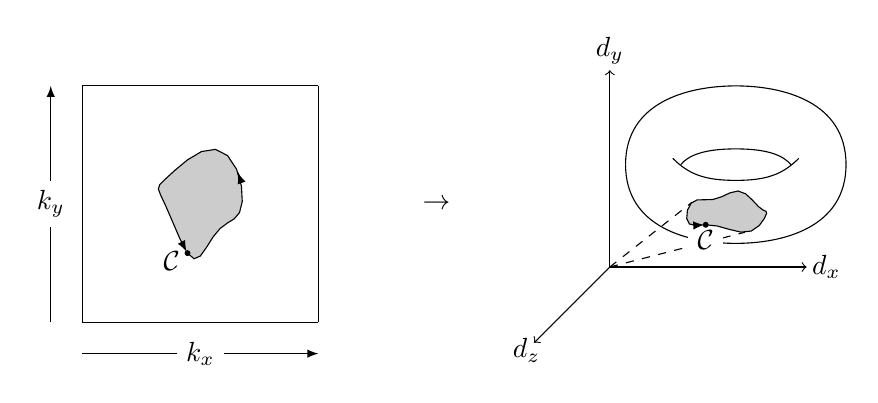
\begin{tikzpicture}

\def \axissize {2.5}
\def \squaresize{1.5}

\def \squarepos{-3}
\def \axisxpos {2.2}
\def \axisypos{-0.8}
\def \arrowdistance {0.4}

\draw (\squarepos - \squaresize , - \squaresize) -- (\squarepos + \squaresize, - \squaresize);
\draw (\squarepos + \squaresize , - \squaresize) -- (\squarepos + \squaresize, + \squaresize);
\draw (\squarepos + \squaresize , + \squaresize) -- (\squarepos - \squaresize, + \squaresize);
\draw (\squarepos - \squaresize , + \squaresize) -- (\squarepos - \squaresize, - \squaresize);

\draw [-latex] (\squarepos - \squaresize  , - \squaresize-\arrowdistance) -- (\squarepos + \squaresize, - \squaresize- \arrowdistance);
\draw [-latex] (\squarepos - \squaresize-\arrowdistance, - \squaresize) -- (\squarepos - \squaresize -\arrowdistance, + \squaresize) ;

\draw node [fill= white] at (\squarepos  , - \squaresize-\arrowdistance) {$k_x$};
\draw node [fill= white] at (\squarepos - \squaresize-\arrowdistance, 0)  {$k_y$};

\draw [-latex, fill= black!20, domain = 0:358] plot ({0.5 * (cos(\x-120) + 0.2 * sin(2*(\x-120))) + \squarepos},{0.6*(sin(\x-120) + 0.2 * cos(3*(\x-190))) });
\draw [-latex, domain = 160:161] plot ({0.5 * (cos(\x-120) + 0.2 * sin(2*(\x-120))) + \squarepos},{0.6*(sin(\x-120) + 0.2 * cos(3*(\x-190))) });

\draw[fill] ({0.5 * (cos(-120) + 0.2 * sin(2*(0-120))) + \squarepos},{0.6*(sin(-120) + 0.2 * cos(3*(-190))) }) circle [radius=0.03];
\draw node at ({0.5 * (cos(-120) + 0.2 * sin(2*(0-120))) + \squarepos -0.2 },{0.6*(sin(-120) + 0.2 * cos(3*(-190))) -0.1 }) {$\mathcal C$};


\draw node at (0,0) {$ \rightarrow$};

\draw [->] (\axisxpos,\axisypos,0) -- (\axisxpos+\axissize,\axisypos,0);
\draw  [->] (\axisxpos,\axisypos,0) -- (\axisxpos,\axisypos+\axissize,0);
\draw  [->] (\axisxpos,\axisypos,0) -- (\axisxpos,\axisypos,\axissize);

\def \donutscale {0.4}
\def \donutx {3.8}
\def \donuty {0.5}

\draw (-3.5*\donutscale+\donutx,0+\donuty) .. controls (-3.5*\donutscale+\donutx,2*\donutscale+\donuty) and (-1.5*\donutscale+\donutx,2.5*\donutscale+\donuty) .. (0+\donutx,2.5*\donutscale+\donuty);
\draw[xscale=-1] (-3.5*\donutscale-\donutx,0+\donuty) .. controls (-3.5*\donutscale-\donutx,2*\donutscale+\donuty) and (-1.5*\donutscale-\donutx,2.5*\donutscale+\donuty) .. (0-\donutx,2.5*\donutscale+\donuty);
\draw[rotate=180] (-3.5*\donutscale-\donutx,0-\donuty) .. controls (-3.5*\donutscale-\donutx,2*\donutscale-\donuty) and (-1.5*\donutscale-\donutx,2.5*\donutscale-\donuty) .. (0-\donutx,2.5*\donutscale-\donuty);
\draw[yscale=-1] (-3.5*\donutscale+\donutx,0-\donuty) .. controls (-3.5*\donutscale+\donutx,2*\donutscale-\donuty) and (-1.5*\donutscale+\donutx,2.5*\donutscale-\donuty) .. (0+\donutx,2.5*\donutscale-\donuty);
\draw (-2*\donutscale+\donutx,.2*\donutscale+\donuty) .. controls (-1.5*\donutscale+\donutx,-0.3*\donutscale+\donuty) and (-1*\donutscale+\donutx,-0.5*\donutscale+\donuty) .. (0+\donutx,-.5*\donutscale+\donuty) .. controls (1*\donutscale+\donutx,-0.5*\donutscale+\donuty) and (1.5*\donutscale+\donutx,-0.3*\donutscale+\donuty) .. (2*\donutscale+\donutx,0.2*\donutscale+\donuty);
\draw (-1.75*\donutscale+\donutx,0+\donuty) .. controls (-1.5*\donutscale+\donutx,0.3*\donutscale+\donuty) and (-1*\donutscale+\donutx,0.5*\donutscale+\donuty) .. (0+\donutx,.5*\donutscale+\donuty) .. controls (1*\donutscale+\donutx,0.5*\donutscale+\donuty) and (1.5*\donutscale+\donutx,0.3*\donutscale+\donuty) .. (1.75*\donutscale+\donutx,0+\donuty);

\def\spposx{3.7}
\def\spposy{-0.1}

\def \angone {280}
\def \angtwo {50}

\draw [dashed] (\axisxpos,\axisypos,0) -- ({0.5 * (cos(\angone-120) + 0.1 * sin(2*(\angone-20))) + \spposx},{0.23*(sin(\angone-120) + 0.2 * cos(4*(\angone-190))) +\spposy});
\draw [dashed]  (\axisxpos,\axisypos,0) -- ({0.5 * (cos(\angtwo-120) + 0.1 * sin(2*(\angtwo-20))) + \spposx},{0.23*(sin(\angtwo-120) + 0.2 * cos(4*(\angtwo-190))) +\spposy});

\draw  node [fill=white]  at ({0.5 * (cos(-120) + 0.1 * sin(2*(-20))) + \spposx},{0.23*(sin(-120) + 0.2 * cos(4*(-190))) +\spposy-0.2}) {$\mathcal C$};

\draw [-latex, fill= black!20, domain = 0:358] plot ({0.5 * (cos(\x-120) + 0.1 * sin(2*(\x-20))) + \spposx},{0.23*(sin(\x-120) + 0.2 * cos(4*(\x-190))) +\spposy});
\draw[fill] ({0.5 * (cos(-120) + 0.1 * sin(2*(-20))) + \spposx},{0.23*(sin(-120) + 0.2 * cos(4*(-190))) +\spposy}) circle [radius=0.03];


\draw node at (\axisxpos+1.1*\axissize,\axisypos,0){$ d_x$};
\draw  node at  (\axisxpos,\axisypos+ 1.1*\axissize,0){$ d_y$};
\draw  node at (\axisxpos,\axisypos, 1.1*\axissize){$d_z$};
\end{tikzpicture}
\end{center}

What about the Chern number? This is found by the integrating the Berry curvature across the whole surface of the torus in d-space. If the embedding of the torus does not contain the origin, then the value of this integral is necessarily zero. Now suppose the torus is embedded such that it contains the origin, then we will have a surface that catches all the Berry flux on its inside and the solid angle subtended is $4\pi$. Thus, the Chern number is $+1$. Similarly, for an embedding that wraps the torus twice around the origin, the subtended flux will correspond to twice the charge of the monopole, leading to a Chern number of $+2$. Thus, we see that the Chern number in this context must be quantised, and can often be read directly from the form of $\textbf d(\textbf k)$ by asking how many times this embedding of the torus wraps the origin.

\subsection{Final Notes}

We close this section with an explanation of the consequences of Chern number in topological insulators.

\subsubsection{Smoothly Deforming the Hamiltonian}

Consider a pair of quantum systems in the same Hilbert space, described by Hamiltonians $\hat H_1$ and $\hat H_2$ which are both gapped at the Fermi level. We might ask: \textit{Is it possible to smoothly deform $\hat H _1$ into $\hat H_2$ without crossing a point where the gap at the Fermi level closes?}

The answer is that it is only possible if the sum of the Chern numbers of the occupied bands of $\hat H_1$ and $\hat H_2$ are the same. This is because the total Chern number of the occupied bands is restricted to only take integer values -- it cannot smoothly change as we deform the Hamiltonian. For the total Chern number to change, we must somewhere cross a point where it is impossible to define a Chern number at all, allowing it to jump discontinuously when we leave that point. This is precisely what happens when the gap at the Fermi level closes. At this point, the occupied bands can no longer be defined as a smooth object in momentum space, since there must be a discontinuity at the band touching point. 

We can illustrate this with the example in \textsection\ref{sec:an_example}. Smoothly deforming the Hamiltonian amounts to changing the shape of the torus embedded in $\textbf d$-space. If any point on the surface of the torus touches the origin, a pair of zero-energy states must appear -- the gap has closed, and the system is conductive. If the band has a Chern number of $+1$, this means that the torus contains the origin. In order to smoothly deform this into a system with zero Chern number, we would need to move the torus such that the origin was now outside. At some point in this deformation the torus surface will have to pass through the origin, creating a conducting Hamiltonian at that point.

Thus, we can classify all Hamiltonians according to the Chern number of their bands. It is always impossible to smoothly deform a Hamiltonian into one with a different Chern number while remaining insulating. Similarly, it is always possible to smoothly deform two Hamiltonians into one another without closing a gap, provided that their bands have identical Chern numbers\footnote{A simple justification for this comes from band flattening. Any Hamiltonian can be smoothly band flattened, where all the states in each band are set to the same energy. Furthermore, for a given set of Chern numbers, all band flattened Hamiltonians (with the same dimensionality) are equivalent. Thus, any two Hamiltonians with identical Chern numbers can be transformed into one another by using the common band flattened Hamiltonian as an intermediate step.}~\cite{avron_homotopy_1983}.

\subsubsection{The Bulk-Boundary Correspondence}

The argument presented above allows us to make a rough justification for why conducting edge states must appear wherever we have a material with nonzero Chern number. Suppose we have a large system where the Hamiltonian is allowed to vary slowly over space, defined by $\hat H (\textbf r)$. In one region this Hamiltonian locally has non-zero Chern number, $\hat H _{\textup{topological}}$, but in a different distant region it locally has zero Chern number, $\hat H _{\textup{trivial}}$. We expect that between these regions the Hamiltonian must be gradually transforming between $\hat H _{\textup{topological}}$ and $\hat H _{\textup{trivial}}$. As we have seen, it is impossible for our Hamiltonian to make this transformation without passing through a conducting region somewhere along the way -- edge states must appear! Exploiting this intuition, one might view the vacuum as having zero Chern number. Thus, we would expect that if a material with non-zero Chern number transforms over space into the vacuum -- that is, it has a boundary -- then conductive states must appear at the boundary. This property of Chern insulators is called the bulk-boundary correspondence \cite{qi_general_2006,hasan_colloquium_2010,qi_topological_2011}.


\subsubsection{Chern Number and Globally Smooth Gauges}\label{sec:chern_smooth_gauge}
Carefully considering the gauge used in Eqn.~\ref{states}, one might notice that there is a discontinuity at $\phi = \pi$ where $e^{i\phi}$ suddenly jumps as you cross over to $\phi = -\pi$. This is no oversight, it is completely impossible to define a globally smooth set of states $\ket{\psi(\textbf{d})}$ for any band that has nonzero Chern number. This is because if $\ket{\psi(\textbf{d})}$ were continuous everywhere, then the Berry connection would also have to be continuous everywhere. Thus, we could invoke Stokes' theorem in Eqn.~\ref{eqn:cont_chern_number}, showing that the Chern number must vanish since the integral is over the whole (closed) manifold. A nonzero Chern number thus relies on there being points where Stokes' theorem cannot be used. In this sense, the Chern number can be regarded as a measure of the amount of discontinuity that \textit{must} be present regardless of the gauge you choose for the space.




\section{The QWZ Model and its Amorphous Counterpart}
For the rest of this document, we will use the Qi-Wu-Zhang (QWZ) model as our example for a topological insulator, first introduced in \cite{qi_topological_2006}. This is because the QWZ model is a simple toy model for a two-dimensional topological insulator with nearest-neighbour interactions on a square lattice.\par
 We work in a similar Hilbert space as that used in \textsection\ref{sec:lattice_bloch}, on a lattice of unit cells indexed by a two dimensional lattice vector $\bf m$, where each cell contains two sites -- the QWZ model has two bands. Thus the Hilbert space of the system is spanned by states of the form
\begin{align}
    \ket{\psi} = \ket{m_x} \otimes \ket{m_y} \otimes \ket{\alpha}.
\end{align}
The lattice has size $(L_x,L_y)$, so we have 
\begin{align}
    m_x \in \{ 0,...,L_x-1\}\\
    m_y \in \{ 0,...,L_y-1\}\\
    \alpha \in \{0,1\}.
\end{align}
The QWZ model is defined by three terms, a hopping between unit cells in the $x$-direction, a hopping in the $y$-direction, and a staggered on-site potential whose strength is determined by a parameter $u$.
\begin{align}
    \hat H &= \sum_{\bf m} \ket{\bf m+ 1_x}\bra{\bf m} \otimes \frac{\sigma_z + i\sigma_x}{2} + h.c. \nonumber \\
    &+ \sum_{\bf m} \ket{\bf m+ 1_y}\bra{\bf m} \otimes \frac{\sigma_z + i\sigma_y}{2} + h.c. \nonumber \\
    &+ \sum_{\bf m} \ket{\bf m}\bra{\bf m} \otimes u\; \sigma_z,
\end{align}
where $1_x$ and $1_y$ represent the unit displacement in their respective directions,
\begin{align}
	1_x = \begin{pmatrix}
	1\\
	0
	\end{pmatrix}, \ 1_y = \begin{pmatrix}
	0\\
	1
	\end{pmatrix}.
\end{align}
\begin{figure}[t]
\begin{center}
 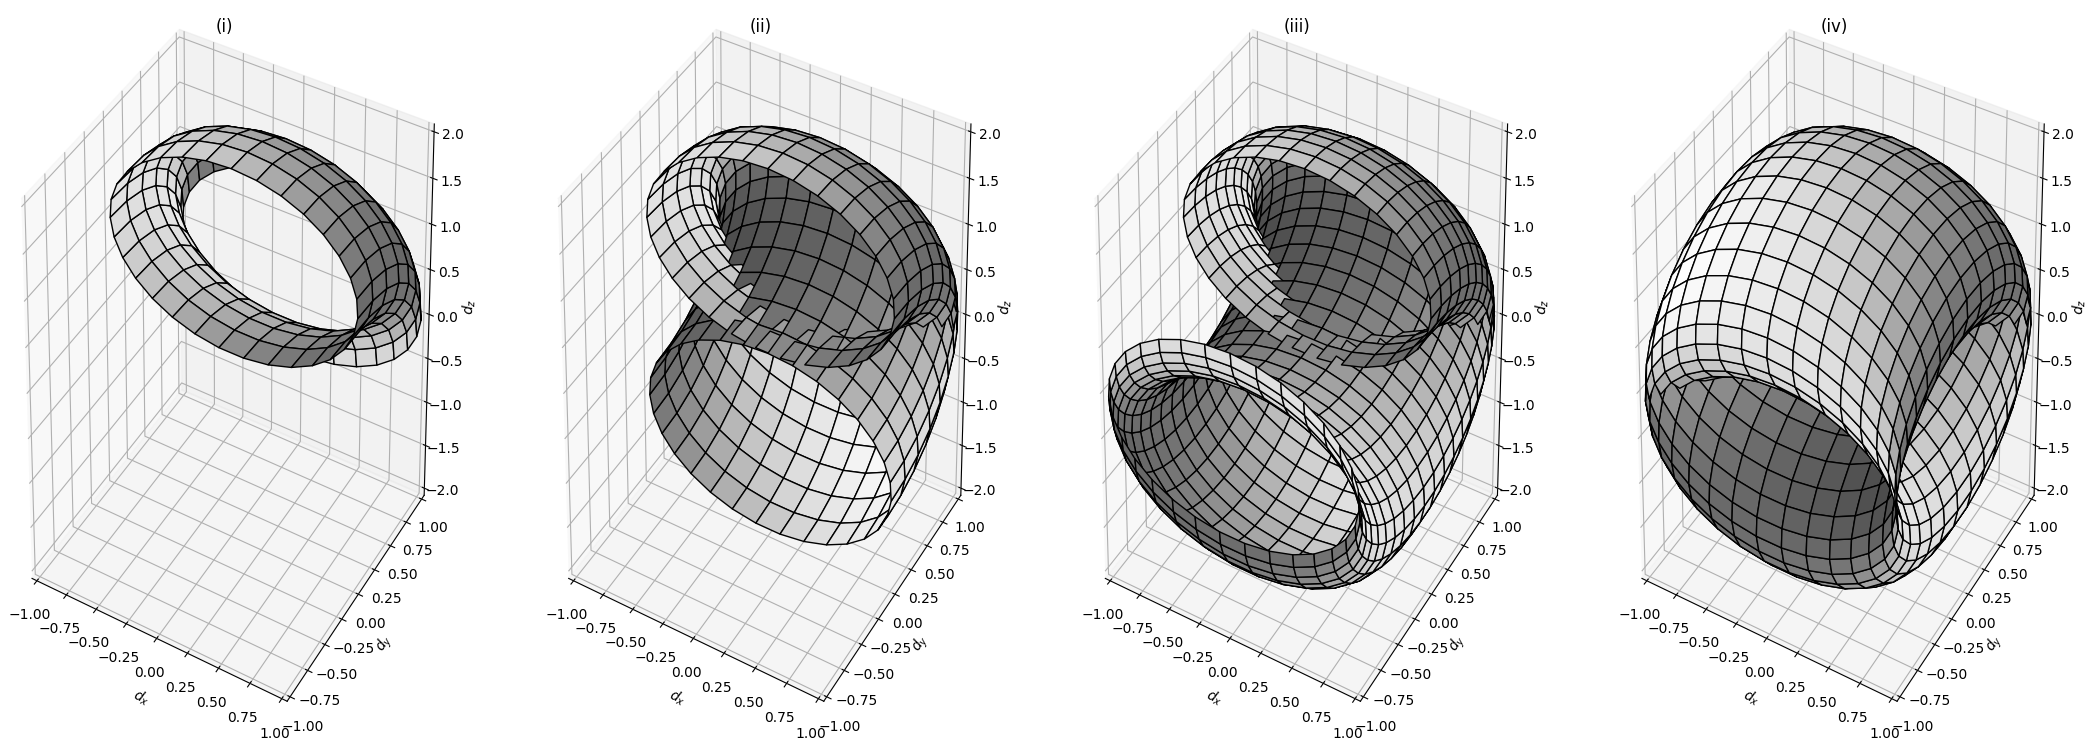
\includegraphics[width=\textwidth]{local_markers_background/figures/QWZ_donut.png}
\caption{The embedding of the Brillouin zone in $\bf d$-space for the QWZ model. This is shown in four progressive cutaways to ensure the internal structure can be seen. In all four images $k_x$ spans the interval $\left ( 0, 2\pi \right ]$, however in (i) $k_y$ spans $\left ( 0, \frac{\pi}{2} \right ]$, in (ii) $k_y$ spans $\left ( 0, \pi \right ]$, in (iii) $k_y$ spans $\left ( 0, \frac{3 \pi}{2} \right ]$, and in (iv) $k_y$ spans $\left ( 0, 2\pi \right ]$. }
\label{fig:QWZ_donut}
\end{center}
\end{figure}
Using Bloch's theorem, we can find the bulk Hamiltonian,
\begin{align}
    \hat H(\bf k) = \begin{pmatrix}
\sin k_x \\ 
\sin k_y\\ 
u + \cos k_x+ \cos k_y
\end{pmatrix} \cdot \bm \sigma.
\end{align}
Here, $k_x$ and $k_y$ determine our position in the Brillouin zone. As explained in \textsection\ref{sec:an_example}, this represents the embedding of a torus in $\bf d$-space, shown in fig. \ref{fig:QWZ_donut}.\par
The $u$-parameter has the effect of translating the torus by a fixed amount in the $z$-direction. From this we can see that the QWZ model only has non-zero Chern number for values of $u$ between -2 and 2. This is because translating the torus by any more than this will place the origin completely outside. The Chern number for the QWZ model is
\begin{align}
Q = \left\{\begin{matrix}
-1 &:&  -2 < u < 0 \\ 
1  &:&  0<u<2\\
0  &:&  \textit{otherwise} 
\end{matrix}\right. ,
\end{align}
not including the points at $u =$ -2, 0 and 2, at which the Chern number is undefined because the band gap closes and the material is conducting. Some example band structures for varying values of $u$ are shown in fig. \ref{fig:QWZ_band_struct}.
\begin{figure}[t]
\begin{center}
 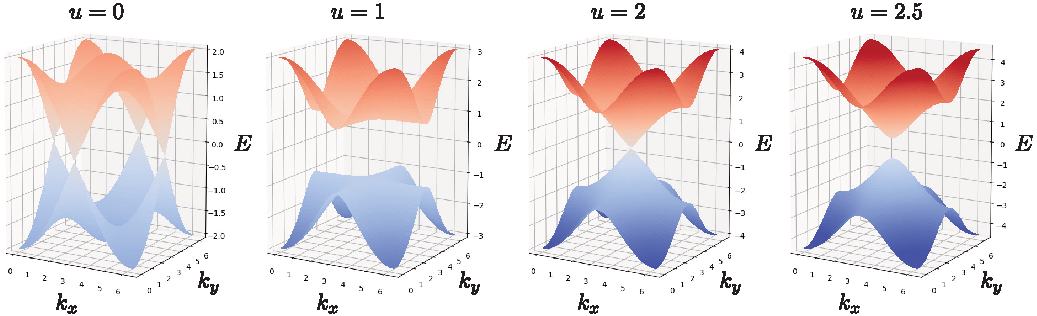
\includegraphics[width=\textwidth]{local_markers_background/figures/QWZ_band_struct}
\caption{Four examples of the band structure of the QWZ model are shown, for varying $u$ values between 0 and 2.5. At $u$ = 0 and 2, the bands touch and Chern number is undefined. At $u$ = 1, Q = +1, and at $u$ = 2.5, Q = 0.}
\label{fig:QWZ_band_struct}
\end{center}
\end{figure}

\subsection{Strip Geometry} \label{sec:QWZ_strip_geometry}
In much of the following discussion, we will be studying the QWZ model in a system with strip geometry. This means that the lattice is periodic and uniform in the $y$-direction, but is allowed to be non-uniform or have open boundaries in the $x$-direction. We will allow $u$ to vary in the $x$-direction, so add a subscript to indicate position-dependence $u \rightarrow u_{m_x}$. We can apply Bloch's theorem in the $y$-direction only, and our eigenstates take the following form,
\begin{align}
    \ket{\psi} = \ket{k_y}\otimes \ket{v_{k_y}^{n,l}},
\end{align}
where $\ket{k_y}$ is a plane wave solution
\begin{align}
    \ket{k_y} =\frac{1}{\sqrt{L_y}} \sum_{m_y} e^{i m_y k_y}\ket{m_y},
\end{align}
and $\ket{v_{k_y}^{n,l}}$ is a $2L_x$-element vector in the remaining part of the Hilbert space $\mathcal H_x \otimes \mathcal H_{\textup{int}} $. The $n$ index labels which band the state is in, and the $l$ index differentiates between the states in each band.
\begin{align}
    n &\in \{0,1\}\\
    l &\in \{ 0, \dots ,L_x -1\}.
\end{align}
The $v$-states are solutions of the semi-bulk Hamiltonian
\begin{align}
    \hat H(k_y) &= \sum_{m_x} \ket{m_x+1}\bra{m_x} \otimes \frac{\sigma_z + i\sigma_x}{2} + h.c.\nonumber \\
    &+ \sum_{m_x} \ket{m_x}\bra{m_x} \otimes \left [ (u_{m_x} + \cos k_y) \; \sigma_z + \sin k_y \; \sigma_y  \right ].
\end{align}
We have effectively reduced our system from a lattice of interacting sites in $x$ and $y$, to a set of chain models in $x$, that are each labelled by a value of $k_y$.
\begin{center}
\input{local_markers_background/figures/lattice_to_chain}
\end{center}
We can rewrite this, in terms of the $2\times2$ matrices $A$ and $B$,
\begin{align}
    A &= (u + \cos k_y) \; \sigma_z + \sin k_y \; \sigma_y,  \\ 
    B &= \frac{\sigma_z + i\sigma_x}{2},
\end{align}
and express our wavevectors in terms of a set of $L_x$ two-element states $\psi_n$
\begin{align}
    \ket{\psi} = \begin{pmatrix}
    \psi_0 \\
    \psi_1 \\
    \vdots \\
    \psi_{L_x -1}
     \end{pmatrix},
\end{align}
to arrive at a set of equations for the eigenvalues of the semi-bulk Hamiltonian.
\begin{align}
    \textup{Bulk:} &\ A\psi_n + B\psi_{n+1} + B^\dag \psi_{n-1} = \lambda \psi_n \\
    \textup{Left Edge:} &\ A\psi_1 + B\psi_{2} = \lambda \psi_1\\
    \textup{Right Edge:} &\ A\psi_{L_x} + B^\dag \psi_{L_x-1}  = \lambda \psi_n
\end{align}
The band structure for this system in both periodic boundaries and strip geometry is shown in fig. \ref{fig:strip_energy}.
\begin{figure}[t]
\begin{center}
 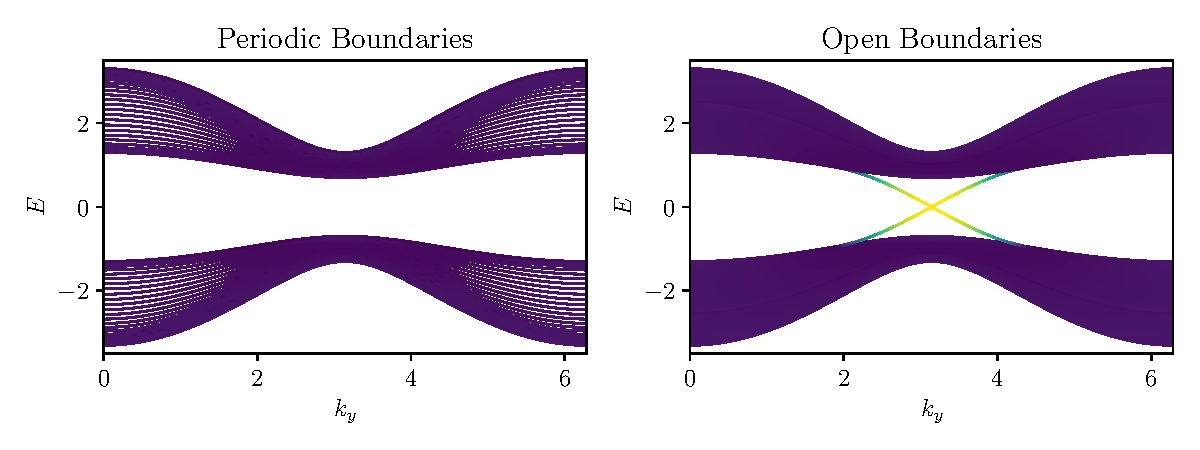
\includegraphics[width=.85\textwidth]{local_markers_background/figures/strip_energy}
\caption{An example band structure for a QWZ model with $u$ = 1.3 and $L_x$ = 30. On the left is the example for periodic boundary conditions, showing two well-separated bands. On the right is the case for open boundary conditions. Two edge states are shown leaving the bulk and crossing the gap, with the descending state being a left edge state, and the ascending state being a right edge state. }
\label{fig:strip_energy}
\end{center}
\end{figure}
We can now look at solving this analytically for the bulk and edge states. We will omit this calculation and print only the form of the results, however a full derivation can be found in appendix \ref{sec:QWZ_model_appendix}. Note that edge states are only present for certain values of $k_y$, which can be seen in figure \ref{fig:strip_energy}, where the edge states only separate from the bulk in a region around $k_y = \pi$. \par
Edge states have the form
\begin{align}
    \ket{\psi^{\textup{left}}_{k_y}} = \sqrt{1-\xi_l^2}\sum_{m=1}^{L_x} \xi_l^{m-1}\ket m \otimes \begin{pmatrix}
    1\\
    -i
    \end{pmatrix}
\end{align}
where 
\begin{align}
    \xi_l &= -u - \cos k_y.
\end{align}
This state has energy
\begin{align}
    E_l &= -\sin k_y.
\end{align}
Similarly, the right edge state is given by
\begin{align}
    \ket {\psi^{\textup{right}}_{k_y}} = \sqrt{1-\xi_r^2} \sum_{m=1}^{L_x} \xi_r^{L_x-m} \ket m \otimes  \begin{pmatrix}
    1\\
    i
    \end{pmatrix}
\end{align}
with the extra conditions
\begin{align}
   	 \xi_r &= -u-\cos k \label{eqn:edge_condition}\\
	E_r &= \sin k.
\end{align}
These edge states are only valid solutions for $k_y$ in the region
\begin{align}
	-1 < u+\cos k_y < 1.
\end{align}
These limits can be seen in fig. \ref{fig:strip_energy}, where the edge states peel away from the bands to cross the energy gap.\par
The bulk states are less straightforward to obtain exact solutions for, we give the general form for them and leave the details to appendix \ref{sec:QWZ_model_appendix}.
\begin{align}
    \ket{\psi^\pm_{k_y} }= \frac{1}{\sqrt{L_x}}\sum \ket{m}  \otimes \left [ \alpha e^{i \theta m} \ket{\phi_{\theta}^{\pm}} + \beta e^{-i \theta m} \ket{\phi_{\theta}^{\pm *}} \right ],
\end{align}
where the exact values of $\theta$, $\alpha$, $\beta$ and $\ket{\phi_{\theta}^{\pm}} $ can be found by solving some fairly unpleasant equations.\par
Here we mention a final caveat, These calculations are only strictly valid in the limit of a large system. This is because we have made the assumption the edge states can be calculated by taking into consideration only one edge and ignoring the effect of the other. The edge states decay exponentially through the system, so we are relying on the assumption that the edge state has effectively decayed to nothing before reaching the other side. When this condition is relaxed the edge states are able to couple to one another. This has a two effects, the first being that at the crossing of edge states, our energy eigenvalues become positive and negative superposition states of both edge states. The other is that the left state coupling to the right state shifts their energy levels such that no states cross $E = 0$ -- there is no longer a crossing of energy levels for the left and right edge states.




\subsection{The Amorphous QWZ Model}


\section{Local Markers}
\subsection{Kitaev's Local Marker}

\subsection{The Bott Index}

\subsection{The Chern Marker}

\bibliographystyle{unsrt}
\bibliography{local_markers/local_markers.bib}

\chapter{The Crosshair Marker}

\chapter{Kitaev's Honeycomb Model}

\chapter{The Amorphous Kitaev Model}

\chapter{The Star Lattice Kitaev-Heisenberg Model}

\chapter{Conclusion and Outlook}

\end{document}